\documentclass[nolayout]{article}

\usepackage[utf8]{inputenc}
\usepackage[english]{babel}
\usepackage{amsmath,amsthm}
\usepackage{geometry}
\usepackage{tikz}
\usetikzlibrary{fit,positioning}
\usepackage[textwidth=4cm,textsize=footnotesize]{todonotes}
\usepackage{fancyhdr}
\pagestyle{fancy}
\usepackage{amssymb,color,bbm,xargs}
\usepackage{graphicx}
\usepackage[active]{srcltx}
\usepackage{ifthen}
\usepackage{enumerate}
\usepackage{dsfont}
\usepackage{subcaption}

\newtheorem{lemma}{Lemma}
\newtheorem{proposition}{Proposition}
\newtheorem{theorem}{Theorem}
\newtheorem{corollary}{Corollary}

\definecolor{lavander}{cmyk}{0,0.48,0,0}
\definecolor{violet}{cmyk}{0.79,0.88,0,0}
\definecolor{burntorange}{cmyk}{0,0.52,1,0}
\definecolor{burntgreen}{cmyk}{0.62,0.44,0.47,0}
\definecolor{burntblue}{cmyk}{0.86,0.30,0.18,0}
\definecolor{palegreen}{cmyk}{0.86,0.30,0.96,0}


\def\sup{\mathrm{sup}}
\def\param{\theta}
\def\paramset{\Theta}
\def\1{\mathds{1}}
\def\rset{\mathbb{R}}
\def\rmd{\mathrm{d}}
\def\eqsp{\,}
\def\Pstar{\mathbb{P}_{\pi_{\star}}}
\def\bayes{\pi_{\star}}
\def\kernel{\mathsf{M}}
\newcommand{\limit}[1]{\underset{#1\to \infty}{\longrightarrow}}
\newcommand{\E}{\mathbb{E}}
\newcommand{\kullback}{\mathsf{L}}
\newcommand{\link}{\leftrightarrow}


\newcommand{\pa}[1]{\left(#1\right)}
\newcommand{\cro}[1]{\left[#1\right]}
\newcommand{\set}[1]{\left\{#1\right\}}
\newcommand{\PE}[1]{\left\lfloor#1\right\rfloor}

\newcommand{\loss}[1]{\ell\pa{#1}}
\newcommand{\Lo}[2]{\ell^{#1}\pa{#2}}

\newcommand{\bN}{\mathbb{N}}
\newcommand{\bP}{\mathbb{P}}
\newcommand{\bR}{\mathbb{R}}
\newcommand{\bZ}{\mathbb{Z}}

\newcommand{\cA}{\mathcal{A}}
\newcommand{\cD}{\mathcal{D}}
\newcommand{\cE}{\mathcal{E}}
\newcommand{\cO}{\mathcal{O}}
\newcommand{\cS}{\mathcal{S}}
\newcommand{\cV}{\mathcal{V}}
\newcommand{\cX}{\mathcal{X}}

\newcommand{\ordermax}[2]{{\mathsf{q}}^{#1}_{#2}}
\newcommand{\remainder}[2]{{\mathsf{r}}^{#1}_{#2}}

\newcommand{\condlik}{k}
\newcommand{\card}{\mathrm{card}}

\newcommand{\MLE}{\widehat{\pi}}

\newcounter{hypH}
\newenvironment{hypH}{\refstepcounter{hypH}\begin{itemize}
\item[{\bf H\arabic{hypH}}]}{\end{itemize}}
\begin{document}
\begin{frontmatter}

\title{Learning latent structure of large random graphs}


\begin{aug}
  \author{\fnms{Roland}  \snm{Diel}\ead[label=e1]{Roland.Diel@unice.fr}},
  \author{\fnms{Sylvain} \snm{Le Corff}\ead[label=e2]{sylvain.le-corff@math.u-psud.fr}}
  \and
  \author{\fnms{Matthieu}  \snm{Lerasle}%
  \ead[label=e3]{matthieu.lerasle@math.u-psud.fr}%
}

  \runauthor{R. Diel et al.}

  \affiliation{Univ. Nice, Univ. Paris-Sud, CNRS, Univ. Paris-Saclay}

  \address{Laboratoire J.A.Dieudonn\'e UMR CNRS-UNS 6621 Universit\'e de Nice Sophia-Antipolis 06108 NICE Cedex 2\\
          \printead{e1}}

  \address{Laboratoire de math\'ematiques d'Orsay, Univ. Paris-Sud, CNRS, Universit\'e Paris-Saclay, 91405 Orsay\\ 
          \printead{e2,e3}}

\end{aug}

\begin{abstract}~In this paper, we estimate the distribution of hidden nodes weights in large random graphs from the observation of very few edges weights. In this very sparse setting, the first non-asymptotic risk bounds for maximum likelihood estimators (MLE) are established. The proof relies on the construction of a graphical model encoding conditional dependencies that is extremely efficient to study $n$-regular graphs obtained using a round-robin scheduling. This graphical model allows to prove geometric loss of memory properties and deduce the asymptotic behavior of the likelihood function. Following a classical construction in learning theory, the asymptotic likelihood is used to define a measure of performance for the MLE. Risk bounds for the MLE are finally obtained by subgaussian deviation results derived from concentration inequalities for Markov chains applied to our graphical model.
\end{abstract}

\begin{keyword}[class=MSC]
\kwd[Primary ]{62G05}
\kwd[; secondary ]{05C80}
\end{keyword}

\begin{keyword}
\kwd{latent variables}
\kwd{random graphs}
\kwd{non-parametric estimation}
\kwd{non-asymptotic risk bounds}
\end{keyword}

\end{frontmatter}


\section{Introduction}
Inference in large random graphs is an important topic of interest due to its applications to many fields such as data science, sociology or neurobiology for instance. This paper focuses on large random graphs whose heterogeneity is described by latent data models. The nodes are associated with latent random weights, independent and with unknown distribution. The only available information is given by random weights associated with few edges in the graph which are independent conditionally on the nodes weights. The objective is to estimate the unknown distribution of the nodes weights from these observations.  This latent data structure is appealing as it may be used to describe graphs in a wide range of applications. In sports tournaments, nodes represent contestants in a championship and each node weight is the ``intrinsic value" of the corresponding player. An edge is drawn between players when they face each others, the result of a contest is the observed edge weight. The problem is to recover from a few games the distribution of the intrinsic values of the players to make early prediction on the issue of the championship  for example.
In social networks, nodes are members and their weights represent the ``popularity" of each member. An edge is drawn between members if a ``suggestion of friendship" has been made to one of them. The observed edge weight is $0$ if these people are not connected and $1$ otherwise. The problem here is to estimate the popularity density in a large population where only a few suggestions of friendship can be made compared to the global size of the network.
In neurobiology, random graphs may be used to model neural functional connectivity inside the brain. In this case, nodes are neurons and their weights represent their efficiency to diffuse neural information. An edge between neurons is drawn if the activity of these neurons is observed simultaneously. The weight of this edge is a score representing the influence that these neurons exercise on each other. The problem is therefore to estimate the functional connectivity density inside the brain from these scores.

The problem studied in this paper has a long history, going back at least to \cite{zemerlo:1929} who considered the problem of \emph{paired comparison} to evaluate performances of medicines. In \cite{zemerlo:1929} and later in  \cite{bradley:terry:1952}, the problem was to recover the weights of a finite number of nodes when the number of measurements on every pair grows to infinity. Further extensions of the so-called Bradley-Terry model have then been studied, see for example \cite{David:1963} for a review. More recently, \cite{Simons_Yao:1999} considered the problem of estimating nodes weights in Bradley-Terry models based on one measurement per pair of nodes when the number $N$ of nodes grows to infinity. This framework led to several developments in computational statistics for the Bradley-Terry model, see \cite{Hun:2004} and \cite{caron:doucet:2012} for various extensions of this original model. 
A related problem was considered in \cite{chatterjee:diaconis:sly:2011} where an edge is inserted between each pair of nodes with a probability depending on the nodes weights. Each node has therefore a random degree and the observed degrees are used to infer nodes weights. When the graph is fully observed, \cite{chatterjee:diaconis:sly:2011} proved that  with a probability of order $1-1/N^2$, there exists a unique maximum likelihood estimator of the nodes weights which is such that the supremum norm of the estimation error is upper bounded by $\sqrt{\log N/N}$. 

This paper strongly departs from these settings where the all graph is observed, even from \cite{YanYangXu:2011} where some edges are missing. 
We consider a very sparse alternative where only very few edges per nodes are observed.
A reason why such a sparse setting has never been considered is probably due to \cite{zemerlo:1929} who proved that the estimation of the weights is actually impossible in the Bradley-Terry model in this situation. 
To overcome this issue, we consider the problem of estimating \emph{the distribution of the weights} and not the weights themselves. 
There are several motivations to adopt this new approach. 
The Bradley-Terry model in ``random environment"  was applied with success to predict the issue of a championship by estimating the probability distribution of the teams weights (strengths) which were assumed to be uniformly distributed, see for example \cite{Sir_Red:2009} and references therein. 
Moreover, \cite{CheDielLer:2017} recently showed that the node with maximal weight can be recovered if the tail of the nodes weights distribution is sufficiently convex. 
More generally, the idea to use a Bayesian estimator when a frequentist approach is not available is rather standard. 
The performances of this estimator highly depend on the prior distribution of the parameters and providing a reasonable prior may have a great impact. 
The study of bayesian estimators with an estimated prior is known as empirical bayes theory \cite{MR0084919} and is currently a subject of intense research, see for example~\cite{MR2724758} for a recent overview. 
The problem presented in this paper can be understood as finding a statistically efficient estimator of the prior to design an empirical bayes estimator for the nodes weights. 
The use of latent variables is also at the heart of mixed effect models widely spread in biostatistics, see \cite{MR3331127}. 

This paper shows the first non-asymptotic risk bounds for non-parametric maximum likelihood estimators (MLE) of the distribution of nodes weights. 
Asymptotic properties of MLE rely heavily on a loss of memory property of the observed random graph. 
This can be analyzed using a graphical model describing the conditional dependencies between nodes and edges. 
This graphical model provides a natural parallel with hidden Markov models \cite{cappe:moulines:ryden:2005} which is used to study the asymptotic behavior of the likelihood, following \cite{DoucMoulines} in particular. 
The limit likelihood defines a natural notion of risk to measure performances of MLE. 
These performances are obtained for finite values of the number $N$ of nodes using concentration inequalities for Markov Chains \cite{dedecker:gouezel:2015}.
The excess risk scales as the entropy of the underlying statistical model (in the sense of Dudley) normalized by a term of order $\sqrt{N}$ when $n$ is fixed and $N\to\infty$. 
From a learning perspective, Dudley's entropy bound is known to be sub-optimal in general, it can be replaced by a majorizing measure bound \cite{Talagrand:2014} if needed since the bound proposed in this paper is derived from a subgaussian concentration inequality for the underlying process, see Eq.~\eqref{eq:subGaussIncr}. 

More generally, we believe that the methodology introduced to prove our results leads the way to exciting research perspectives in various fields. 
For example, identifiability of non-parametric hidden Markov models with finite state spaces was established very recently along with the first convergence properties of estimators of the unknown distributions, see  \cite{decastro:gassiat:lacour:2016} for a penalized least-squares estimator of the emission densities,  \cite{decastro:gassiat:lecorff:2017,vernet:2015,vernet:2017} for consistent estimation of the posterior distributions of the states and posterior concentration rates for the parameters  or \cite{lehericy:2017} for order estimation.
However, very few theoretical results are available for the non-parametric estimation of general state spaces hidden Markov models. 
The arguments leading to our risk bound may probably be extended to this framework. 
In computational statistics, bayesian estimators of nodes weights have been studied in Bradley-Terry models and other extensions \cite{caron:doucet:2012}. 
Designing new algorithms to compute MLE of the prior would therefore be of great interest to derive empirical bayes estimators of these weights. 

The paper is organized as follows. 
Section~\ref{sec:setting} details the model and the maximum likelihood estimator of  the unknown weights distribution.
Section~\ref{sec:CondDep} presents preliminary results underlying our analysis. A graphical model encoding conditional dependencies in the original graph is built. The round-robin algorithm, a widely spread method in sports tournaments that  builds sparse graphs for which our graphical model is stationary, is also presented. Our main results are finally given in Section~\ref{sec:main}. Convergence of the likelihood is established when the number $N$ of nodes grows to $+\infty$ and risk bounds for the MLE are provided. 
Section~\ref{sec:round:robin} to \ref{sec:MainProofs} are devoted to the proofs of these results. Section~\ref{sec:round:robin} proves the fundamental properties of the graphical model associated with round-robin graphs.
Section~\ref{sec:ProbTools} proves the probabilistic tools required to establish the main results. These tools might be of independent interest, they are presented as independent results and hold for stationary processes with conditional dependencies encoded in the graphical model. 
Proofs of the main results are finally gathered in Section~\ref{sec:MainProofs}.


\section{Setting}
\label{sec:setting}
\subsection{Random graphs with latent variables}
Let $n$, $N$ denote two positive integers and let $(\{1,\ldots,N\},E^{n,N})$ be a connected $n$-regular graph. 
Let $V_1,\ldots,V_N$ denote independent and identically distributed (i.i.d.) random variables taking values in a measurable set $\cV$ with common (unknown) distribution $\bayes$.  For all $\{i,j\}\in E^{n,N}$, the observation $X_{i,j}$ takes values in a discrete set $\cX$ and conditionally on $V=(V_1,\ldots,V_N)$, the random variables $(X_{i,j})_{(i,j)\in E^{n,N}}$ are independent and such that the conditional distribution of $X_{i,j}$ is given by $\condlik: \cX\times\cV\times\cV\to[0,1]$:
\begin{equation*}
%\label{eq:conditional:ind}
\bP(X_{i,j}=x|V)=\condlik(x,V_i,V_j)\eqsp.
\end{equation*}
%where for every vector $a\in \bR^p$ and every subset $B\subset [p]=\{1,\ldots,p\}$, $a_{B}=\{a_i,\;i\in B\}$. 
This framework encompasses the following models.


\begin{Example}[Bradley-Terry model \cite{bradley:terry:1952}]
In this example, $\cV=\rset_+^*$, $\cX=\{0,1\}$ and for all $x\in\cX$,
\[
k(x,V_i,V_j) = \left(\frac{V_i}{V_i+V_j}\right)^x\left(\frac{V_j}{V_i+V_j}\right)^{1-x}\eqsp.
\]
\end{Example}
\begin{Example}[Extensions of Bradley-Terry model]
In \cite{caron:doucet:2012}, the authors proposed several algorithms to perform Bayesian inference for generalized Bradley-Terry models which fit our framework.
\begin{enumerate}[-]
\item The Bradley-Terry model with home advantage introduces an additional parameter $\theta>0$ to measure the home-field advantage. In this case, $\cV=\rset_+^*$, $\cX=\{0,1\}$ and, if the player $i$ is home, for all $x\in\cX$,
\[
k(x,V_i,V_j)= \left(\frac{\theta V_i}{\theta V_i+V_j}\right)^x\left(\frac{V_j}{\theta V_i+V_j}\right)^{1-x}\eqsp.
\]
\item The Bradley-Terry model with ties \cite{rao:kupper:1967} introduces an additional parameter $\theta>1$, $\cV=\rset_+^*$, $\cX=\{-1,0,1\}$ and
\[
k(1,V_i,V_j)= \frac{V_i}{V_i+ \theta V_j}\quad\mbox{and}\quad k(0,V_i,V_j)= \frac{(\theta^2-1) V_i V_j}{\left(\theta V_i+V_j\right)\left( V_i+\theta V_j\right)}\eqsp.
\]
\end{enumerate}
\end{Example}
\begin{Example}[Random graphs with a given degree sequence]
\cite{chatterjee:diaconis:sly:2011} considers random graphs such that, for all $1\le i <j\le N$, an edge is inserted between players $i$ and $j$ with probability $V_iV_j/(1+V_iV_j)$ where $(V_1,\ldots,V_N)$ are parameters to be estimated using the degrees of the vertices in the observed graph. Such random graphs fit our framework with $\cV=\rset_+^*$, $\cX=\{0,1\}$ ($X_{i,j}=0$ in our framework representing $\{i,j\}\notin E$ in theirs) and for all $1\le i <j\le N$, $x\in\cX$,
\[
k(x,V_i,V_j) = \left(\frac{V_iV_j}{1+V_iV_j}\right)^x\left(\frac{1}{1+V_iV_j}\right)^{1-x}\eqsp.
\]
\end{Example}
\subsection{Maximum likelihood estimator}
The weights $X^{n,N}=(X_{i,j})_{(i,j)\in E^{n,N}}$ are observed and  the objective is to infer the distribution $\bayes$ of the hidden variables $V=(V_1,\ldots,V_N)$ from these observations. Let $\Pi$ be a set of probability measures on $\cV$. For all $\pi\in\Pi\cup\{\bayes\}$, the joint distribution of $(X^{n,N},V)$ is given by
%\textcolor{cyan}{Sylvain : j'ai mis $\mathbb{P}$ pour la vraisemblance pour etre homogene avec la suite... J'ai fait une commande au cas o\`u \c ca ne vous plairait pas !}
%\textcolor{red}{Matthieu : Comme tu as eu raison}
\begin{equation}
\label{eq:jointlaw}
\likelihood{n,N}{\pi}(x^{n,N},A)=\int\un{A}(v)\prod_{(i,j) \in E^{n,N}}k(x^{n,N}_{i,j},v_{i},v_j)\pi^{\otimes N}(\rmd v)\eqsp.
\end{equation}
Using the convention $\log 0=-\infty$, the log-likelihood is given, for all $\pi\in\Pi\cup\{\bayes\}$, by
\[
\Lo{n,N}{\pi} = \log\,\likelihood{n,N}{\pi}(X^{n,N})\eqsp,\qquad\text{where}\qquad  \likelihood{n,N}{\pi}(X^{n,N})=\likelihood{n,N}{\pi}(X^{n,N},\cV)\eqsp.
\]
In this paper, $\bayes$ is estimated by the standard maximum likelihood estimator $\MLE^{n,N}$ defined as any maximizer of the log-likelihood:
\[
\MLE^{n,N}\in \argmax_{\pi\in\Pi}\{\Lo{n,N}{\pi}\}\eqsp.
\]


\section{Round-robin graphical model}
\label{sec:CondDep}
%
Section~\ref{sec:GM} details a graphical model encoding the conditional dependences between the random variables $(X^{n,N},V)$. This graphical model is studied in the particular case of round-robin graphs in Section~\ref{sec:RRscheduling}. 
%
\subsection{Graphical model}\label{sec:GM}
%
Let $d^{n,N}_0$ denote the graph distance in $(\{1,\ldots,N\},E^{n,N})$, that is $d^{n,N}_0(i,j)$ is the minimal length of a path between nodes $i$ and $j$. Write $\{V_1,\ldots,V_N\}=\cup_{q=0}^{N}V^{n,N}_{q}$, where $V^{n,N}_{0}= \{V_1\}$ and, for any $q\ge 1$, $V^{n,N}_{q}$ is the set of $V_i$ such that $d^{n,N}_0(1,i)=q$. 
%Lemma~\ref{lem:ElementsAtDistanceq} describes the elements in the sets $V_{q}^{n,N}$, $q\ge 1$, when players meet according to the round-robin scheduling. 
Let $\ordermax{n}{N}+1$ denote the maximal distance between $1$ and $i\in\{1,\ldots,N\}$:
\[
\ordermax{n}{N}+1 = \max_{1\le i\le N}\,d^{n,N}_0(1,i)\eqsp.
\]
\begin{enumerate}[-]
\item For all $1\le q \le \ordermax{n}{N}+1$, let 
\[
X^{n,N}_{q\link q}=\{X_{i,j} : \{i,j\}\in E^{n,N},\; i\in V_q^{n,N},\; j\in V_q^{n,N}\}\eqsp.
\]
The set $X^{n,N}_{q\link q}$ gathers all $X_{i,j}$ such that $i$ and $j$ satisfy $d^{n,N}_0(V_1,V_i) = d^{n,N}_0(V_1,V_j)=q$.
\item For all $0\le q \le \ordermax{n}{N}$, let 
\[
X^{n,N}_{q\link q+1}=\{X_{i,j} : \{i,j\}\in E^{n,N},\; i\in V_q^{n,N},\; j\in V_{q+1}^{n,N}\}\eqsp.
\]
Likewise, the set $X^{n,N}_{q\link q+1}$ gathers all $X_{i,j}$ such that $d^{n,N}_0(V_1,V_i) = q$ and $d^{n,N}_0(V_1,V_j)=q+1$.
\end{enumerate} 
Finally, for any $0\le q \le \ordermax{n}{N}$, let 
\begin{align*}
X_{q}^{n,N}& = X_{q \link q+1}^{n,N}\cup X_{q+1\link q+1}^{n,N}\eqsp.
\end{align*}
By \eqref{eq:jointlaw} the joint distribution of 
$(V_q^{n,N})_{0\le q\le \ordermax{n}{N}+1}$ and $(X^{n,N}_{q})_{0\le q \le \ordermax{n}{N}}$ may be factorized using the conditional independence between some subsets of these variables. For all $0\le q \le \ordermax{n}{N}$, and all $\pi\in\Pi$,
\[
\bP^{n,N}_{\pi}\left(X^{n,N}_{q}\middle| V,X^{n,N}_{0:q-1}\right) = \bP^{n,N}_{\pi}\left(X^{n,N}_{q}\middle| V^{n,N}_{q},V^{n,N}_{q+1}\right)=\prod_{\{i,j\} :X_{i,j}\in X^{n,N}_{q}}\condlik\left(X_{i,j},V_i,V_j\right)\eqsp.
\]
These conditional dependences are represented in the graphical model of Figure~\ref{fig:generic:graphicalmodel}, where graph separations represent conditional independences. For all $0\le q \le \ordermax{n}{N}$ any path between $X^{n,N}_{q}$ and other vertices except $V_q^{n,N}$ and $V_{q+1}^{n,N}$ goes through $V_{q}^{n,N}$ or $V_{q+1}^{n,N}$ which means that $X^{n,N}_{q}$ is independent of all other nodes given $V_q^{n,N}$ and $V_{q+1}^{n,N}$. 

\begin{figure}[h!]
\centering
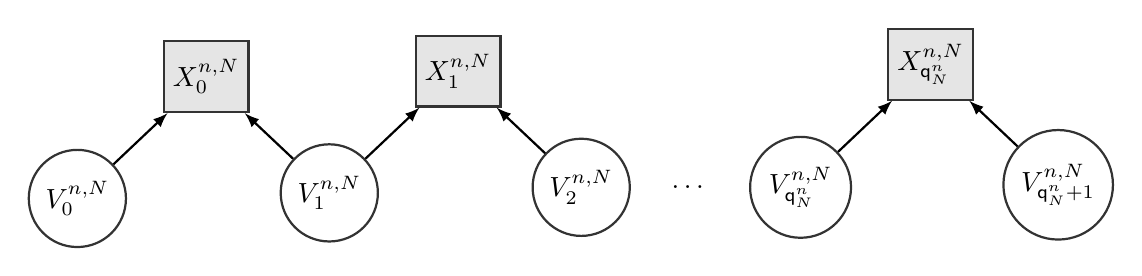
\begin{tikzpicture}
\tikzstyle{player}=[circle, minimum size = 12mm, thick, draw =black!80, node distance = 8mm]
\tikzstyle{game}=[rectangle, minimum size = 9mm, thick, draw =black!80, node distance = 9mm]
\tikzstyle{connect}=[-latex, thick]
\tikzstyle{box}=[rectangle, draw=black!100]
\node[player] (v0){$V^{n,N}_{0}$};
\node[game, fill = black!10] (X01) [above right =of v0] {$X^{n,N}_{0}$};
\node[player] (v1) [below right=of X01] {$V^{n,N}_{1}$ };

\path (v0) edge [connect] (X01);  
\path (v1) edge [connect] (X01);  

\node[game, fill = black!10] (X12) [above right =of v1] {$X^{n,N}_{1}$};
\node[player] (v2) [below right=of X12] {$V^{n,N}_{2}$ };

\path (v1) edge [connect] (X12);  
\path (v2) edge [connect] (X12);  

\node[player] (vq) [right=of v2,xshift = .7cm] {$V^{n,N}_{\ordermax{n}{N}}$ };

\path (v2) -- node[auto=false]{\ldots}  (vq); 


\node[game, fill = black!10] (Xq1) [above right =of vq] {$X^{n,N}_{\ordermax{n}{N}}$};
\node[player] (vq1) [below right=of Xq1] {$V^{n,N}_{\ordermax{n}{N}+1}$ };


\path (vq1) edge [connect] (Xq1); 
\path (vq) edge [connect] (Xq1); 

\end{tikzpicture}
\caption{Graphical model of a paired comparisons based contest.}
\label{fig:generic:graphicalmodel}
\end{figure}

\subsection{Round-Robin Scheduling}\label{sec:RRscheduling}
There is a large variety of $n$-regular graphs (even up to permutations of the indices), the results of this paper are obtained for the graph built using the round-robin scheduling. At time $t=1$, this algorithm pairs nodes according to Figure~\ref{fig:robin:day1}, that is $2i-1$ is paired with $2i$, for all $i\in[N/2]$. At time $t=2$, a node is fixed and all others are rotated clockwise as described in Figure~\ref{fig:robin:move}. Node $1$ does not move, $2$ takes the place of $3$, each odd integer $2i-1<N-1$ takes the place of $2i+1$, $N-1$ takes the place of $N$ and each even integer $2i>2$ takes the place of $2(i-1)$. Then, each node is paired with the new node it faces as in Figure~\ref{fig:robin:day2}. At each time $t> 2$, each node moves once according to the round-robin step detailed in Figure~\ref{fig:robin:move} and is paired with the new node it faces. The round-robin graph denoted by $E^{n,N}_{{\rm RR}}$ studied in detail in this paper contains all pairs collected in the first $n$ rotations of the round-robin algorithm. 

\begin{figure}[h!]
\begin{subfigure}{\textwidth}
  \centering
  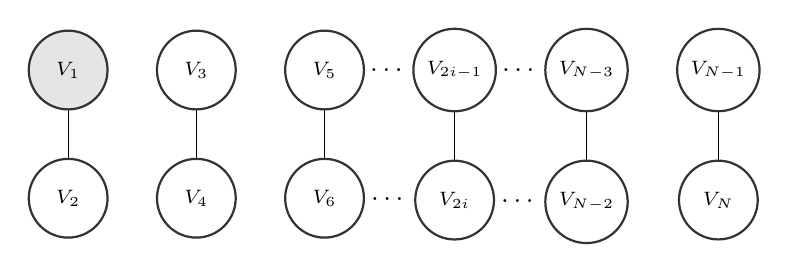
\begin{tikzpicture}
\tikzstyle{main}=[circle, minimum size = 10mm, thick, draw =black!80, node distance = 6mm]
\tikzstyle{connect}=[-latex, thick]
\tikzstyle{box}=[rectangle, draw=black!100]
\node[main, fill = black!10] (v1){$\scriptstyle V_1$ };
\node[main] (v3) [right=of v1] {$\scriptstyle V_3$ };
\node[main] (v5) [right=of v3] {$\scriptstyle V_5$ };
\node[main] (v7) [right=of v5] {$\scriptstyle {V_{2i-1}}$};
\node[main] (v9) [right=of v7] {$\scriptstyle{V_{N-3}}$};
\node[main] (v11) [right=of v9] {$\scriptstyle{V_{N-1}}$};
\node[main] (v2) [below=of v1] {$\scriptstyle V_2$};
\node[main] (v4) [below=of v3] {$\scriptstyle V_4$};
\node[main] (v6) [below=of v5] {$\scriptstyle V_6$};
\node[main] (v8) [below=of v7] {$\scriptstyle{V_{2i}}$};
\node[main] (v10) [below=of v9] {$\scriptstyle{V_{N-2}}$};
\node[main] (v12) [below=of v11] {$\scriptstyle{V_{N}}$};
\draw (v1) -- (v2);
\draw (v3) -- (v4);
\draw (v5) -- (v6);
\draw (v7) -- (v8);
\draw (v9) -- (v10);  
\draw (v11) -- (v12);     
\path (v5) -- node[auto=false]{\ldots}  (v7); 
\path (v7) -- node[auto=false]{\ldots}  (v9); 
\path (v6) -- node[auto=false]{\ldots}  (v8); 
\path (v8) -- node[auto=false]{\ldots}  (v10);    
\end{tikzpicture}
\caption{Round-robin, $t=1$.}
\label{fig:robin:day1}
\end{subfigure}

\vspace{.7cm}

\begin{subfigure}{\textwidth}
  \centering
  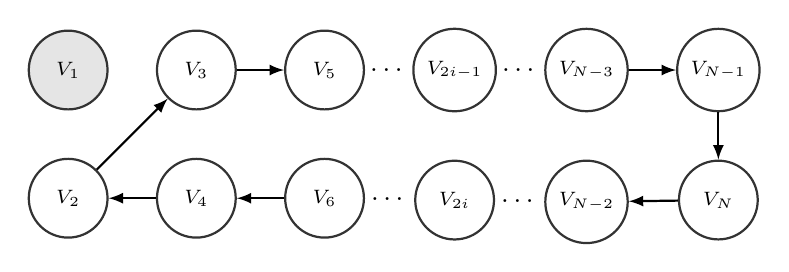
\begin{tikzpicture}
\tikzstyle{main}=[circle, minimum size = 10mm, thick, draw =black!80, node distance = 6mm]
\tikzstyle{connect}=[-latex, thick]
\tikzstyle{box}=[rectangle, draw=black!100]
\node[main, fill = black!10] (v1){$\scriptstyle V_1$ };
\node[main] (v3) [right=of v1] {$\scriptstyle V_3$ };
\node[main] (v5) [right=of v3] {$\scriptstyle V_5$ };
\node[main] (v7) [right=of v5] {$\scriptstyle{V_{2i-1}}$};
\node[main] (v9) [right=of v7] {$\scriptstyle{V_{N-3}}$};
\node[main] (v11) [right=of v9] {$\scriptstyle{V_{N-1}}$};
\node[main] (v2) [below=of v1] {$\scriptstyle V_2$};
\node[main] (v4) [below=of v3] {$\scriptstyle V_4$};
\node[main] (v6) [below=of v5] {$\scriptstyle V_6$};
\node[main] (v8) [below=of v7] {$\scriptstyle{V_{2i}}$};
\node[main] (v10) [below=of v9] {$\scriptstyle{V_{N-2}}$};
\node[main] (v12) [below=of v11] {$\scriptstyle{V_{N}}$};
\path (v2) edge [connect] (v3);   
\path (v4) edge [connect] (v2);  
\path (v3) edge [connect] (v5);  
\path (v6) edge [connect] (v4); 
\path (v9) edge [connect] (v11); 
\path (v11) edge [connect] (v12);   
\path (v12) edge [connect] (v10);   
\path (v5) -- node[auto=false]{\ldots}  (v7); 
\path (v7) -- node[auto=false]{\ldots}  (v9); 
\path (v6) -- node[auto=false]{\ldots}  (v8); 
\path (v8) -- node[auto=false]{\ldots}  (v10);    
\end{tikzpicture}
\caption{Round-robin moves.}
\label{fig:robin:move}
\end{subfigure}

\vspace{.7cm}

\begin{subfigure}{\textwidth}
\centering
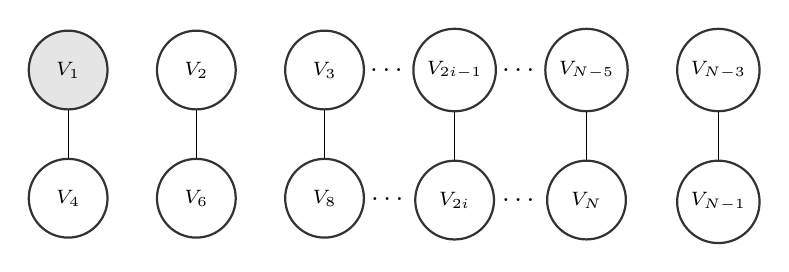
\begin{tikzpicture}
\tikzstyle{main}=[circle, minimum size = 10mm, thick, draw =black!80, node distance = 6mm]
\tikzstyle{connect}=[-latex, thick]
\tikzstyle{box}=[rectangle, draw=black!100]
\node[main, fill = black!10] (v1){$\scriptstyle V_1$ };
\node[main] (v3) [right=of v1] {$\scriptstyle V_2$ };
\node[main] (v5) [right=of v3] {$\scriptstyle V_3$ };
\node[main] (v7) [right=of v5] {$\scriptstyle{V_{2i-1}}$};
\node[main] (v9) [right=of v7] {$\scriptstyle{V_{N-5}}$};
\node[main] (v11) [right=of v9] {$\scriptstyle{V_{N-3}}$};
\node[main] (v2) [below=of v1] {$\scriptstyle V_4$};
\node[main] (v4) [below=of v3] {$\scriptstyle V_6$};
\node[main] (v6) [below=of v5] {$\scriptstyle V_8$};
\node[main] (v8) [below=of v7] {$\scriptstyle {V_{2i}}$};
\node[main] (v10) [below=of v9] {$\scriptstyle{V_{N}}$};
\node[main] (v12) [below=of v11] {$\scriptstyle{V_{N-1}}$};
\draw (v1) -- (v2);
\draw (v3) -- (v4);
\draw (v5) -- (v6);
\draw (v7) -- (v8);
\draw (v9) -- (v10);  
\draw (v11) -- (v12);     
\path (v5) -- node[auto=false]{\ldots}  (v7); 
\path (v7) -- node[auto=false]{\ldots}  (v9); 
\path (v6) -- node[auto=false]{\ldots}  (v8); 
\path (v8) -- node[auto=false]{\ldots}  (v10);    
\end{tikzpicture}
\caption{Round-robin, $t=2$.}
\label{fig:robin:day2}
\end{subfigure}
\caption{First two days using the round-robin algorithm.}
\end{figure}

\noindent
Lemma~\ref{lem:RR:stat} gathers results on the graphical model of Figure~\ref{fig:generic:graphicalmodel} when $E^{n,N}=E^{n,N}_{\text{RR}}$ that are central in our analysis.

\begin{lemma}\label{lem:RR:stat} 
Let $n,N\ge1$ and $(\{1,\ldots,N\},E^{n,N}_{\text{RR}})$ be the round-robin graph. Assume that $2\le n<N/4$. Then, $\ordermax{n}{N}$ is the quotient of the Euclidean division of $N/2-1$ by $n-1$, that is $N/2-1= \ordermax{n}{N}(n-1)+\remainder{n}{N}$ where $0\le \remainder{n}{N}<n-1$. Moreover, $(V^{n,N}_{q},X^{n,N}_{q})_{2\le q\le \ordermax{n}{N}-1}$ is a stationary Markov chain such that for all $2\le q\le \ordermax{n}{N}-1$,
\[
\absj{V^{n,N}_{q}} = 2(n-1)\eqsp, \quad \absj{X^{n,N}_{q}} = n(n-1)\eqsp.
\]
\end{lemma}
\noindent Lemma~\ref{lem:RR:stat} is proved in Section~\ref{sec:round:robin}.

\section{Main results}\label{sec:main}
Section~\ref{sec:ConvLikelihood} computes the limit likelihood function and define a natural risk function to evaluate the performances of the MLE. Risk bounds for the MLE are obtained in Section~\ref{sec:RBMLE} using non-asymptotic concentration inequalities for Markov chains.


\subsection{Convergence of the likelihood}\label{sec:ConvLikelihood}
The problem being reduced to the analysis of the graphical model of Figure~\ref{fig:generic:graphicalmodel}, convergence results follow from the geometrically decaying mixing rates of the conditional law of $(V^{n,N}_{k})_{0\le k \le \ordermax{n}{N}+1}$ given $X^{n,N}_{q:\ordermax{n}{N}-1}$ for any $0\le q< \ordermax{n}{N}$. These rates derive from the following assumption.
\begin{hypH}
\label{assum:strongmix}
There exists $\varepsilon>0$ such that for all $x\in\cX, \pi\in\Pi\cup\{\bayes\}$ and $v_1,v_2 \in \mathrm{supp}(\pi)$, $\condlik(x,v_{1},v_2)\ge\varepsilon$.
%\begin{equation}
%\label{eq:bound:likelihood}
%\varepsilon\le \condlik(x,v_{1},v_2)(\le 1)\eqsp.
%\end{equation}
\end{hypH}
When $E^{n,N}=E^{n,N}_{\text{RR}}$, by Lemma~\ref{lem:RR:stat}, 
%the cells $V^{n,N}_i$ for $i\in \{2,\ldots \ordermax{n}{N}\}$ have equal cardinalities and the cells $X_{i}^{n,N}$ for $i\in \{2,\ldots,\ordermax{n}{N}-1\}$ also. This ensures that 
the joint sequence $(X^{n,N}_q,V^{n,N}_q)_{2\le q \le \ordermax{n}{N}-1}$ is a stationary Markov chain which may be extended to a stationary process indexed by $\mathbb{Z}$ with the same transition kernel. This extension is denoted by $({\bf X^{n}},{\bf V^{n}})$. 

%These computations are tedious and therefore postponed to Section~\ref{sec:round:robin}. 
Define also the shift operator $\shift$ on $(\cX^{n(n-1)})^{\mathbb{Z}}$ by $(\shift x)_k = x_{k+1}$ for all $k\in\mathbb{Z}$ and all $x\in (\cX^{n(n-1)})^{\mathbb{Z}}$.

\begin{theorem}\label{thm:ConvVrais}
Assume H\ref{assum:strongmix} holds and $(\{1,\ldots,N\},E^{n,N}_{\text{RR}})$ is the round-robin graph. 
%Let $(X^{n,N}_{q})_{ q>1}$ denote a stationary extension of $(X^{n,N}_{q})_{2\le q\le \ordermax{n}{N}-1}$. 
There exists a function $\ell_{\pi}^{n}$ such that for all $q\ge 2$,
%$(\log p_{\pi}^{n,N}(X_{q}^{n,N}|X_{q+1:\ordermax{n}{N}-1}^{n,N}))_{N\ge 1}$ converges uniformly in $\pi\in\Pi$, $\Pstar$-a.s, 
\begin{equation}\label{eq:bound:loglik}
\sup_{\pi\in\Pi} \absj{\log \likelihood{n,N}{\pi}(X_{q}^{n,N}|X_{q+1:\ordermax{n}{N}-1}^{n,N})-\ell_{\pi}^{n}(\shift^q{\bf X^{n}})}\limit{N}0,\qquad \Pstar\mbox{-a.s}\eqsp. 
\end{equation}
%Define for any $q\in\mathbb{Z}$, $\ell_{q,n}^\infty(\pi)=\ell_{\pi}^{n}(\shift^q{\bf X^{n,N}})$,
Moreover, for all $\pi\in\Pi$, $\Pstar$-a.s.  and in $\mathrm{L}^1(\Pstar)$,
\begin{equation}\label{eq:ApproxRisk}
\frac{1}{\ordermax{n}{N}}\log \likelihood{n,N}{\pi}\left(X^{n,N}\right) \limit{N} \kullback^n_{\bayes}(\pi) = \E_{\bayes}\left[\ell_{\pi}^{n}({\bf X^{n}})\right]\eqsp. 
\end{equation}
\end{theorem}

Theorem~\ref{thm:ConvVrais} establishes convergence to the limit likelihood $\kullback^n_{\bayes}(\pi)$ when the number of nodes $N$ goes to $\infty$ while $n$ remains fixed. The rate of almost sure convergence $\ordermax{n}{N}$ is proportional to $N$ by Lemma~\ref{lem:RR:stat}. Eq~\eqref{eq:ApproxRisk} is the key to understand the definition of the risk function used in the next section. We proceed as in Vapnick's learning theory \cite{MR1641250, MR0474638} described now to establish a parallel with our framework. Let $Y,Y_1,\ldots,Y_N$ denote i.i.d. observations in $\cY$, let $F$ denote a set of parameters, and let $\ell: F\times\cY\to\rset$ denote a loss function. The empirical risk minimizer is defined in this context by
\[
\hat f_N^{\text{ERM}}=\argmin_{f\in F}\sum_{i=1}^N\ell(f,Y_i)\eqsp.
\]
If $\E[\ell(f,Y_1)]<\infty$ for all $f\in F$, the risk of any $f\in F$ is measured by the \emph{excess risk}  \cite{MassartNedelec2006}
\[
R(f)=\E\cro{\ell(f,Y)}-\E\cro{\ell(f^*,Y)}\eqsp,
\]
where $Y$ is a copy of $Y_1$, independent of $Y_{1},\ldots,Y_N$ and $f^*$ is the minimizer of $\E[\ell(f,Y)]$ over $F$. Note that when $\E[\ell(f,Y_1)]<\infty$, for all $f\in F$ the normalized empirical criterion satisfies almost surely,
\[
\frac1N\sum_{i=1}^N\ell(f,Y_i)\to \E[\ell(f,Y_1)]\eqsp.
\]
Therefore the excess risk $R(f)$ is the difference between normalized asymptotic empirical criteria in $f$ and its minimizer. In this paper, the MLE minimizes $-\log \likelihood{n,N}{\pi}\left(X^{n,N}\right)$, which, properly normalized converges to $-\kullback^n_{\bayes}(\pi)$. This suggests to define the risk function
\begin{equation}\label{def:ExcessRisk}
R^n_{\bayes}(\pi)=\kullback^{n}_{\bayes}(\bayes)-\kullback^{n}_{\bayes}(\pi),\qquad \forall\pi\in\Pi\eqsp. 
\end{equation}
By Proposition~\ref{prop:max:likelihood}, $\bayes$ is actually a minimizer of $-\kullback^{n}_{\bayes}(\pi)$ over $\Pi\cup\{\bayes\}$. 
Therefore, $R^n_{\bayes}$ is the excess risk associated with the likelihood function.

\subsection{Risk bounds for the MLE}\label{sec:RBMLE}
The following theorem provides non-asymptotic deviation bounds for the excess risk of the MLE. This is the main result of this paper. 
\begin{theorem}
\label{th:risk}
Assume H\ref{assum:strongmix} holds and $(\{1,\ldots,N\},E^{n,N}_{\text{RR}})$ is the round-robin graph. For any probability measures $\pi$ and $\pi'$, let 
 \begin{equation}
 \label{eq:def:d}
 d(\pi,\pi')=
\begin{cases}
 \|\pi-\pi'\|_{\mathsf{tv}}\log\pa{\frac1{\|\pi-\pi'\|_{\mathsf{tv}}}}&\text{if} \;\|\pi-\pi'\|_{\mathsf{tv}}\le e^{-1}\eqsp,\\
  \|\pi-\pi'\|_{\mathsf{tv}}&\text{if} \;\|\pi-\pi'\|_{\mathsf{tv}}\ge e^{-1}\eqsp.
\end{cases}
\end{equation}
Assume that $\Pi$ is a compact set for the topology induced by $d$ and let $\mathsf{N}(\Pi\cup\{\bayes\},d,\epsilon)$ be the minimal number of balls of $d$-radius $\epsilon$ necessary to cover $\Pi\cup\{\bayes\}$. Then, there exists $c>0$ such that, for any $t>0$,
\[
\likelihood{n,N}{\bayes}\pa{R^{n}_{\bayes}(\MLE^{n,N})>\frac{cn\varepsilon^{-6n^2}}{\sqrt{N}}\cro{\int_0^{+\infty}\sqrt{\log \mathsf{N}(\Pi\cup\{\bayes\},d,\epsilon)}\rmd\epsilon+t}}\le e^{-t^2}\eqsp.
\] 
\end{theorem}
Theorem~\ref{th:risk} is proved in Section~\ref{sec:proofs:risk}.
It provides the first non-asymptotic risk bounds for any estimator in a very sparse setting where the number of edges $n$ observed for each node can be very small compared to the number of nodes $N$. 
It proves that the problem studied in this paper is fundamentally different from the problem of nodes weights estimation that is usually considered, at least in Bradley-Terry models. 
While estimating nodes weights is only possible when $n$ is as large as $N$ \cite{zemerlo:1929, Simons_Yao:1999, YanYangXu:2011}, some information on their distribution may be recovered when $n\ll N$. 
This difference is extremely relevant in sports tournaments for example, it means that one can start to make prediction on the final issue of a championship only after a few weeks, while predictions on the issue of each game can only be made when half the year has passed.

The distance $d$ defined in \eqref{eq:def:d} used to measure the entropy of $\Pi$ is not intuitive. However, it is easy to check that $d(\pi,\pi')\le C_\alpha\norm{\pi-\pi'}_{\text{tv}}^{1-\alpha}$ for any $\alpha>0$. It follows that, for any class $\Pi$ with polynomial entropy for the total variation distance, that is such that $\mathsf{N}(\Pi\cup\{\bayes\},\norm{\cdot}_{\text{tv}},\epsilon)\lesssim \epsilon^D$ for small $\epsilon$, Dudley's entropy integral for distance $d$ satisfies 
\[
\int_0^{+\infty}\sqrt{\log \mathsf{N}(\Pi\cup\{\bayes\},d,\epsilon)}\rmd\epsilon\lesssim_{\alpha} \sqrt{D}\eqsp.
\]
Therefore, ``slow rates" of convergence are obtained for the MLE. The polynomial growth $\mathsf{N}(\Pi\cup\{\bayes\},\norm{\cdot}_{\text{tv}},\epsilon)\lesssim \epsilon^D$ is extremely standard, see \cite[p271--274]{MR1652247} for various examples where this assumption is satisfied and our result applies. 
On the other hand, ``fast" rates of convergence remain an open question. 
In particular, the margin condition \cite{MR1765618} required to prove such rates would hold if the total variation distance between distributions of the nodes weights was bounded from above by the excess risk derived from the asymptotic of the likelihood. 




The remaining of the paper is devoted to the proof of the main results. Section~\ref{sec:round:robin} proves Lemma~\ref{lem:RR:stat}, describing precisely the structure of the graphical model given in Figure~\ref{fig:generic:graphicalmodel} in the case of a round-robin scheduling. Then, Section~\ref{sec:ProbTools} establishes central tools in the analysis of the likelihood of stationary processes whose conditional dependences are encoded in the graphical model of Figure~\ref{fig:generic:graphicalmodel}. These results, that might be of independent interest, are therefore stated as independent lemmas.  These tools are finally used in Section~\ref{sec:MainProofs} to prove the main theorems.

\section{Round-robin scheduling}
\label{sec:round:robin}
This section details the sets $V_q^{n,N}$ and $X_q^{n,N}$ for $0\le q\le \ordermax{n}{N}+1$ when $E^{n,N}=E^{n,N}_{\text{RR}}$ (cf. Figures~\ref{fig:robin:day1}-\ref{fig:robin:day2}). In the following, notations for nodes and their weights are identified, i.e. $i$ is identified with $V_i$ for all $1\le i \le N$. Lemma~\ref{lem:RR:stat} follows directly from Lemma~\ref{lem:ElementsAtDistanceq} and Lemma~\ref{lem:cardX} below. To prove these lemmas, consider the following notations.
%ide a more detailed graphical model specific to the round-robin scheduling (cf. Figure~\ref{fig:robin:graphicalmodel}) define: 
\begin{gather*}
\cE=\{4x-1,4x : x\in[\PE{N/4}]\}\quad\mbox{and}\quad \cO=[N]\setminus\cE\eqsp.
\end{gather*}
The notation $\cE$ (resp $\cO$) comes from the fact that $\cE$ (resp $\cO$) contains all $i$ paired with $1$ after an \emph{even} (resp \emph{odd}) number $n\le N/4$ of rotations of the round-robin scheduling. For all $1\le q\le \ordermax{n}{N}$, let
\[
V_{q,e}^{n,N}= V_{q}^{n,N}\cap \cE\quad\mbox{and}\quad V_{q,o}^{n,N}= V_{q}^{n,N}\cap \cO\eqsp.
\]
%The corresponding observations $X_{q\link q,e}^{n,N}$, $X_{q\link q,o}^{n,N}$ for $1\le q\le \ordermax{n}{N}$ and $X_{q\link q+1,e}^{n,N}$, $X_{q\link q+1,e}^{n,N}$ for $0\le q\le \ordermax{n}{N}$ are described in Figure~\ref{fig:robin:graphicalmodel}.
%\begin{align*}
%\mbox{For\,all\,} 1\le q\le \ordermax{n}{N}\,,\,X_{q\link q,e}^{n,N}&= \{X_{i,j}\;;\; V_i\in V_{q,e}^{n,N}\quad\mbox{and}\quad V_j\in V_{q,e}^{n,N}\}\\
%X_{\ordermax{n}{N}+1\link \ordermax{n}{N}+1,e}^{n,N}&= \{X_{i,j}\;;\; V_i\in V_{\ordermax{n}{N}+1}^{n,N}\quad\mbox{and}\quad V_j\in V_{\ordermax{n}{N}+1}^{n,N}\}\eqsp,\\
%X_{q\link q+1,e}^{n,N}&= \{X_{i,j}\;;\; V_i\in V_{q,e}^{n,N}\quad\mbox{and}\quad V_j\in V_{q+1,e}^{n,N}\}\eqsp,\\
%\end{align*}


\begin{lemma}\label{lem:ElementsAtDistanceq} 
Let $n,N\ge1$ and $(\{1,\ldots,N\},E^{n,N}_{\text{RR}})$ be the round-robin graph. Assume that $2\le n<N/4$ and let $N/2-1= \ordermax{n}{N}(n-1)+\remainder{n}{N}$ where $0\le \remainder{n}{N}<n-1$. Then, 
\begin{equation}\label{def:V1}
V_{1}^{n,N}=\{V_{2x} : x=1,\ldots,n\}\eqsp, 
\end{equation}
and, for any $2\le q \le \ordermax{n}{N}$, 
\begin{multline}\label{def:Vq}
V_{q}^{n,N}=\{V_{2x+1} : x\in[(q-2)(n-1)+1,(q-1)(n-1)]\}\\
\cup\{V_{2x} : x\in[2+(q-1)(n-1),1+q(n-1)]\}\eqsp.
\end{multline}
Furthermore,
\begin{multline}\label{def:Vq01'}
V_{\ordermax{n}{N}+1}^{n,N}=\{V_{2x+1} : x\in[(\ordermax{n}{N}-1)(n-1)+1,\ordermax{n}{N}(n-1)+\remainder{n}{N}]\}\\
\cup\{V_{2x} : x\in[2+\ordermax{n}{N}(n-1),1+\remainder{n}{N}+\ordermax{n}{N}(n-1)]\}\eqsp.
\end{multline}
Therefore, $|V_{0}^{n,N}|=1$, $|V_{1}^{n,N}|=n$ and for all $2\le q\le\ordermax{n}{N}$, $\absj{V_{q}^{n,N}}=2(n-1)$.
\end{lemma}
\begin{proof} To ease the reading of this proof, one can check its arguments on Figures~\ref{fig:groups:r0} and~\ref{fig:groups:r1}.

\begin{figure}[h!]
\centering
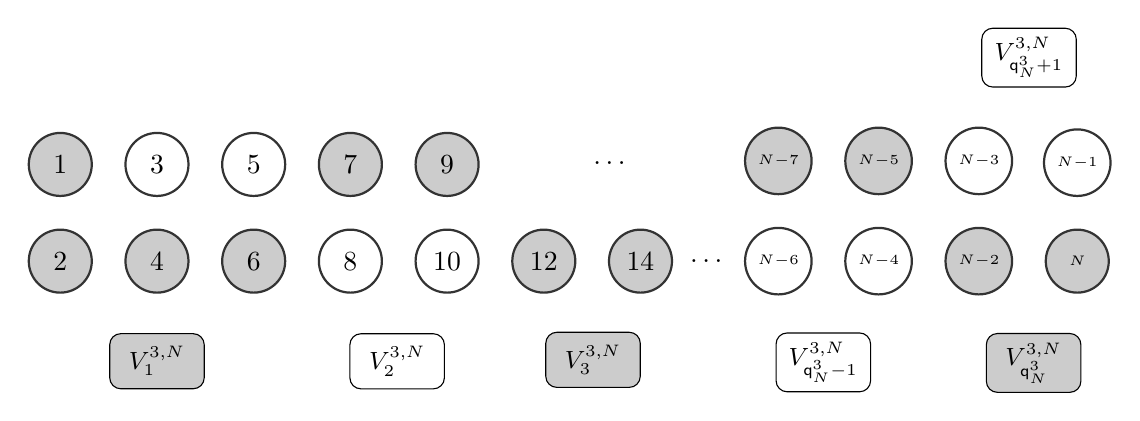
\begin{tikzpicture}
\tikzstyle{main}=[circle, minimum size = 8mm, thick, draw =black!80, node distance = 4mm]
\tikzstyle{V6}=[draw =black!80,circle,minimum size = 8mm, thick,node distance = 4mm,palegreen,bottom color=palegreen!30,top color= white, text=violet]
\tikzstyle{V5}=[draw =black!80,circle,minimum size = 8mm, thick,node distance = 4mm,burntblue,bottom color=burntblue!30,top color= white, text=violet]
\tikzstyle{V4}=[draw =black!80,circle,minimum size = 8mm, thick,node distance = 4mm, text=black]
\tikzstyle{V3}=[draw =black!80,circle,minimum size = 8mm, thick,node distance = 4mm,lavander,bottom color=lavander!30,top color= white, text=violet]
\tikzstyle{V2}=[draw =black!80,circle,minimum size = 8mm, thick,node distance = 4mm,burntorange,bottom color=burntorange!30,top color= white, text=violet]
\tikzstyle{V1}=[draw =black!80,circle,minimum size = 8mm, thick,node distance = 4mm, fill = black!20, text=black]

\tikzstyle{legend_V1}=[node distance = 5mm,rectangle, rounded corners, thin, fill = black!20, draw, text=black,
                           minimum width=1.2cm, minimum height=0.7cm]
\tikzstyle{legend_V2}=[node distance = 8.8mm,rectangle, rounded corners, thin,bottom color=burntorange!30, ,top color= white,
                           burntorange, fill= white, draw, text=violet,
                           minimum width=1.2cm, minimum height=0.7cm]
\tikzstyle{legend_V3}=[node distance = 8.8mm,rectangle, rounded corners, thin,bottom color=lavander!30, ,top color= white,
                           lavander, fill= white, draw, text=violet,
                           minimum width=1.2cm, minimum height=0.7cm]      
\tikzstyle{legend_V4}=[node distance = 8.8mm,rectangle, rounded corners, thin, fill= white, draw, text=black,
                           minimum width=1.2cm, minimum height=0.7cm]                                                                                 
\tikzstyle{legend_V5}=[node distance = 8.8mm,rectangle, rounded corners, thin,bottom color=burntblue!30, ,top color= white,
                           burntblue, fill= white, draw, text=violet,
                           minimum width=1.2cm, minimum height=0.6cm]     
\tikzstyle{legend_V6}=[node distance = 4.8mm,rectangle, rounded corners, thin,bottom color=palegreen!30, ,top color= white,
                           palegreen, fill= white, draw, text=violet,
                           minimum width=1.2cm, minimum height=0.6cm]                                                             
\tikzstyle{connect}=[-latex, thick]
\tikzstyle{box}=[rectangle, draw=black!100]
\node[V1] (v1){$1$ };
\node[V4] (v3) [right=of v1] {$3$ };
\node[V4] (v5) [right=of v3] {$5$ };
\node[V1] (v7) [right=of v5] {$7$ };
\node[V1] (v9) [right=of v7] {$9$ };
\node[V1] (v2) [below=of v1] {$2$};
\node[V1] (v4) [below=of v3] {$4$};
\node[V1] (v6) [below=of v5] {$6$};
\node[V4] (v8) [below=of v7] {$8$};
\node[V4] (v10) [below=of v9] {$10$};
\node[V1] (v12) [right=of v10] {$12$};
\node[V1] (v14) [right=of v12] {$14$};
\node[V4] (v16) [right=of v14,xshift= .5cm] {${\scriptscriptstyle N-6}$};
\node[V4] (v18) [right=of v16] {${\scriptscriptstyle N-4}$};
\node[V1] (v20) [right=of v18] {${\scriptscriptstyle N-2}$};
\node[V1] (v22) [right=of v20] {${\scriptscriptstyle N}$};
\node[V1] (v11) [above=of v16] {${\scriptscriptstyle N-7}$};
\node[V1] (v13) [above=of v18] {${\scriptscriptstyle N-5}$};
\node[V4] (v15) [above=of v20] {${\scriptscriptstyle N-3}$};
\node[V4] (v17) [above=of v22] {${\scriptscriptstyle N-1}$};
   
\path (v14) -- node[auto=false]{\ldots}  (v16); 
\path (v9) -- node[auto=false]{\ldots}  (v11); 
 
\node[legend_V1] [below=of v4] {\small{\textsc{$V_1^{3,N}$}}};
\node[legend_V4] [below right=of v6,xshift= .3cm] {\small{\textsc{$V_2^{3,N}$}}};
\node[legend_V1] [below right=of v10,xshift= .6cm,yshift=-.25cm] {\small{\textsc{$V_3^{3,N}$}}};
\node[legend_V4] [below right=of v14,xshift= .8cm,yshift=.01cm] {\small{\textsc{$V_{\ordermax{3}{N}-1}^{3,N}$}}};
\node[legend_V1] (leg) [below right=of v18,xshift= .7cm,yshift=-.25cm] {\small{\textsc{$V_{\ordermax{3}{N}}^{3,N}$}}};
\node[legend_V4] [above right =of v15,xshift= -.9cm] {\small{\textsc{$V_{\ordermax{3}{N}+1}^{3,N}$}}};
\end{tikzpicture}
\caption{Elements of $\cV^{3,N}$, case $\remainder{3}{N} = 0$.}
\label{fig:groups:r0}
\end{figure}

\begin{figure}[h!]
\centering
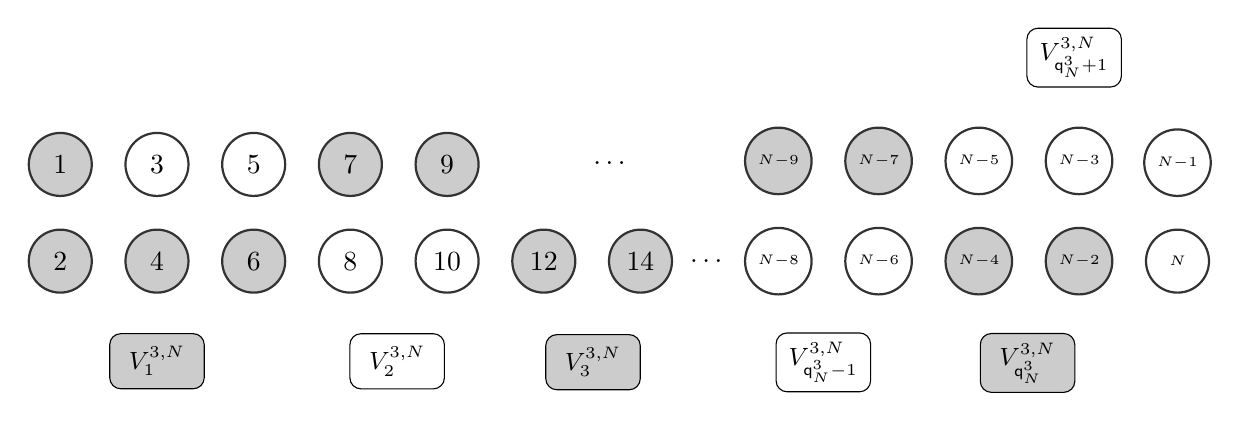
\begin{tikzpicture}
\tikzstyle{main}=[circle, minimum size = 8mm, thick, draw =black!80, node distance = 4mm]
\tikzstyle{V6}=[draw =black!80,circle,minimum size = 8mm, thick,node distance = 4mm,palegreen,bottom color=palegreen!30,top color= white, text=violet]
\tikzstyle{V5}=[draw =black!80,circle,minimum size = 8mm, thick,node distance = 4mm,burntblue,bottom color=burntblue!30,top color= white, text=violet]
\tikzstyle{V4}=[draw =black!80,circle,minimum size = 8mm, thick,node distance = 4mm, text=black]
\tikzstyle{V3}=[draw =black!80,circle,minimum size = 8mm, thick,node distance = 4mm,lavander,bottom color=lavander!30,top color= white, text=violet]
\tikzstyle{V2}=[draw =black!80,circle,minimum size = 8mm, thick,node distance = 4mm,burntorange,bottom color=burntorange!30,top color= white, text=violet]
\tikzstyle{V1}=[draw =black!80,circle,minimum size = 8mm, thick,node distance = 4mm, fill = black!20, text=black]

\tikzstyle{legend_V1}=[node distance = 5mm,rectangle, rounded corners, thin, fill = black!20, draw, text=black,
                           minimum width=1.2cm, minimum height=0.7cm]
\tikzstyle{legend_V2}=[node distance = 8.8mm,rectangle, rounded corners, thin,bottom color=burntorange!30, ,top color= white,
                           burntorange, fill= white, draw, text=violet,
                           minimum width=1.2cm, minimum height=0.7cm]
\tikzstyle{legend_V3}=[node distance = 8.8mm,rectangle, rounded corners, thin,bottom color=lavander!30, ,top color= white,
                           lavander, fill= white, draw, text=violet,
                           minimum width=1.2cm, minimum height=0.7cm]      
\tikzstyle{legend_V4}=[node distance = 8.8mm,rectangle, rounded corners, thin, fill= white, draw, text=black,
                           minimum width=1.2cm, minimum height=0.7cm]                                                                                 
\tikzstyle{legend_V5}=[node distance = 8.8mm,rectangle, rounded corners, thin,bottom color=burntblue!30, ,top color= white,
                           burntblue, fill= white, draw, text=violet,
                           minimum width=1.2cm, minimum height=0.6cm]     
\tikzstyle{legend_V6}=[node distance = 4.8mm,rectangle, rounded corners, thin,bottom color=palegreen!30, ,top color= white,
                           palegreen, fill= white, draw, text=violet,
                           minimum width=1.2cm, minimum height=0.6cm]                                                             
\tikzstyle{connect}=[-latex, thick]
\tikzstyle{box}=[rectangle, draw=black!100]
\node[V1] (v1){$1$} ;
\node[V4] (v3) [right=of v1] {$3$};
\node[V4] (v5) [right=of v3] {$5$};
\node[V1] (v7) [right=of v5] {$7$};
\node[V1] (v9) [right=of v7] {$9$};
\node[V1] (v2) [below=of v1] {$2$};
\node[V1] (v4) [below=of v3] {$4$};
\node[V1] (v6) [below=of v5] {$6$};
\node[V4] (v8) [below=of v7] {$8$};
\node[V4] (v10) [below=of v9] {$10$};
\node[V1] (v12) [right=of v10] {$12$};
\node[V1] (v14) [right=of v12] {$14$};
\node[V4] (v24) [right=of v14,xshift= .5cm] {${\scriptscriptstyle N-8}$};
\node[V4] (v16) [right=of v24] {${\scriptscriptstyle N-6}$};
\node[V1] (v18) [right=of v16] {${\scriptscriptstyle N-4}$};
\node[V1] (v20) [right=of v18] {${\scriptscriptstyle N-2}$};
\node[V4] (v22) [right=of v20] {${\scriptscriptstyle N}$};
\node[V1] (v19) [above=of v24] {${\scriptscriptstyle N-9}$};
\node[V1] (v11) [above=of v16] {${\scriptscriptstyle N-7}$};
\node[V4] (v13) [above=of v18] {${\scriptscriptstyle N-5}$};
\node[V4] (v15) [above=of v20] {${\scriptscriptstyle N-3}$};
\node[V4] (v17) [above=of v22] {${\scriptscriptstyle N-1}$};
 
\path (v14) -- node[auto=false]{\ldots}  (v24); 
\path (v9) -- node[auto=false]{\ldots}  (v19); 

\node[legend_V1] [below=of v4] {\small{\textsc{$V_1^{3,N}$}}};
\node[legend_V4] [below right=of v6,xshift= .3cm] {\small{\textsc{$V_2^{3,N}$}}};
\node[legend_V1] [below right=of v10,xshift= .6cm,yshift=-.28cm] {\small{\textsc{$V_3^{3,N}$}}};
\node[legend_V4] [below right=of v14,xshift= .8cm,yshift=.01cm] {\small{\textsc{$V_{\ordermax{3}{N}-1}^{3,N}$}}};
\node[legend_V1] (leg) [below right=of v18,xshift= -.65cm,yshift=-.25cm] {\small{\textsc{$V_{\ordermax{3}{N}}^{3,N}$}}};
\node[legend_V4] [above right =of v15,xshift= -1.6cm] {\small{\textsc{$V_{\ordermax{3}{N}+1}^{3,N}$}}};
\end{tikzpicture}
\caption{Elements of $\cV^{3,N}$, case $\remainder{3}{N} = 1$.}
\label{fig:groups:r1}
\end{figure}

\noindent
We proceed by induction on $q$.
The definition of $V_{1}^{n,N}$ given by \eqref{def:V1} is straightforward. Then, $V_{2}^{n,N}$ contains:
\begin{enumerate}[-]
\item all $V_i$ paired with some $V_j\in V_{1}^{n,N}$ on the first rotation of the algorithm besides $V_1$ that does not belong to $V_{2}^{n,N}$. These are all  $\{V_{2x+1} : x=1,\ldots,n-1\}$ ;
\item All $V_i$ paired with $V_2$ and $V_4$ that are not in $V_{0}^{n,N}\cup V_{1}^{n,N}$. After $n$ rotations of the round-robin algorithms, all $V_i$ paired with $V_2$ are $\{V_1,V_{4x+2} : x=1,\ldots,n-1\}$ and those with $V_4$ are $\{V_1,V_3,V_{4x} : x=2,\ldots,n-2\}$. 
\end{enumerate}
Therefore, 
\[
V_{2}^{n,N}\supset \{V_{2x+1} : x=1,\ldots,n-1\}\cup\{V_{2x} : x=n+1,\ldots,2n-1\}\eqsp.
\]
On the other hand, by induction,  for all $i\notin \{N-2x+1, x=1,\ldots,2(n-1)\}\cup \{2x : x=1,\ldots, 2n-1\}$,
\begin{gather}
\notag\text{if }i \text{ is odd, it is paired with }\{V_{i+4x+1} : x=0,\ldots n-1\}\eqsp,\\
\label{eq:Opponents}\text{if }i \text{ is even, it is paired with }\{V_{i-4x-1} : x=0,\ldots,n-1\}\eqsp.
\end{gather}
This implies that there is no even number $i\ge 4n$ nor odd number $i>2n-1$ such that $V_i\in V_{2}^{n,N}$, which yields:
\begin{equation*}
 V_{2}^{n,N}= \{V_{2x+1} : x=1,\ldots,n-1\}\cup\{V_{2x} : x=n+1,\ldots,2n-1\}\eqsp.
\end{equation*}
\eqref{def:Vq} is obtained by induction using the same arguments and \eqref{def:Vq01'} is a direct consequence of the round-robin algorithm. 
The last claim follows by noting that for all $q\in[2,\ordermax{n}{N}]$,
\[
|V_{q,e}^{n,N}|=|V_{q,o}^{n,N}|=n-1\eqsp.
\]
Indeed, one of the following cases holds.
\begin{enumerate}[-]
\item $n-1=2p$ for some $p\in \bN$. In this case, 
\[
|\{j: V_j\in V_{q,e}^{n,N},j\in 2\bZ\}|=|\{i : V_i\in V_{q,e}^{n,N},i\in 2\bZ+1\}|=p\eqsp.
\]
\item $n-1=2p+1$ for some $p\in \bN$. In this case, either 
\[
|\{j: V_j\in V_{q,e}^{n,N},j\in 2\bZ\}|=p,\qquad\text{and}\qquad |\{i : V_i\in V_{q,e}^{n,N},i\in 2\bZ+1\}|=p+1\eqsp,
\]
or 
\[
|\{j: V_j\in V_{q,e}^{n,N},j\in 2\bZ\}|=p+1,\qquad\text{and}\qquad |\{i : V_i\in V_{q,e}^{n,N},i\in 2\bZ+1\}|=p\eqsp.
\]
\end{enumerate}
\end{proof}
%The most important result of Lemma~\ref{lem:ElementsAtDistanceq} regarding the decomposition of the likelihood is \eqref{def:Vq} which provides the general expression of nodes in $V_{q}^{n,N}$, for $2\le q\le \ordermax{n}{N}$. This is illustrated in Figures~\ref{fig:groups:r0}-\ref{fig:groups:r1}.
%
%
%Finally, $\cV^{n,N}=\{V_0^{n,N},V_{\ordermax{n}{N}+1}^{n,N},V_{q,e}^{n,N},V_{q,o}^{n,N},q=1,\ldots,\ordermax{n}{N}\}$. 

\begin{lemma}
\label{lem:cardX}
Let $n,N\ge1$ and $(\{1,\ldots,N\},E^{n,N}_{\text{RR}})$ be the round-robin graph.  Then, for all $2\le q\le \ordermax{n}{N}-1$, 
\[
|X_{q}^{n,N}| = n(n-1)\eqsp.
\]
\end{lemma}
\begin{proof}
The proof essentially consists in building the graphical model of Figure~\ref{fig:robin:graphicalmodel} from  the one displayed in Figure~\ref{fig:generic:graphicalmodel}. 


\begin{figure}[h!]
\centering
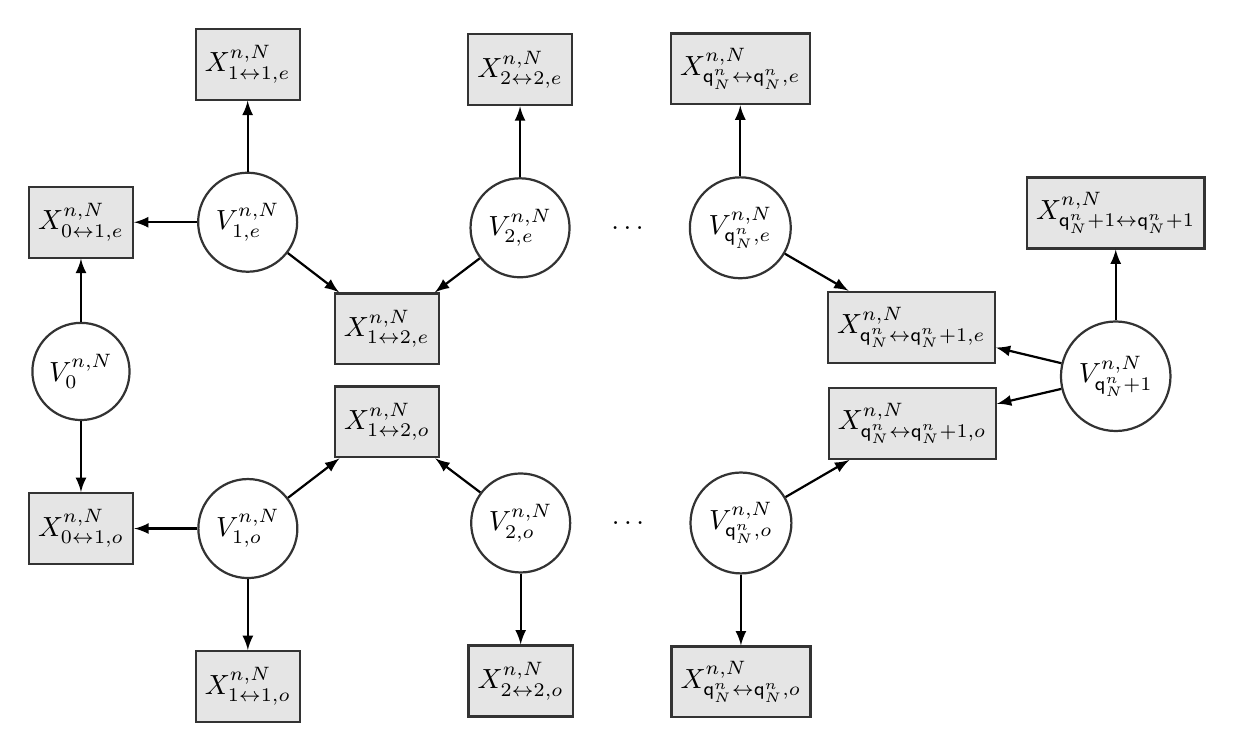
\begin{tikzpicture}
\tikzstyle{player}=[circle, minimum size = 9mm, thick, draw =black!80, node distance = 8mm]
\tikzstyle{game}=[rectangle, minimum size = 9mm, thick, draw =black!80, node distance = 9mm]
\tikzstyle{connect}=[-latex, thick]
\tikzstyle{box}=[rectangle, draw=black!100]
\node[game, fill = black!10] (v1){$X^{n,N}_{0\link1,e}$};
\node[player] (v2) [below=of v1] {$V^{n,N}_{0}$};
\node[game, fill = black!10] (v3) [below=of v2] {$X^{n,N}_{0\link1,o}$};
\node[player] (v4) [right=of v1] {$V^{n,N}_{1,e}$ };
\node[player] (v5) [right=of v3] {$V^{n,N}_{1,o}$ };
\node[game, fill = black!10] (v6) [above=of v4] {$X^{n,N}_{1\link1,e}$};
\node[game, fill = black!10] (v7) [below=of v5] {$X^{n,N}_{1\link1,o}$};

\path (v2) edge [connect] (v3);  
\path (v2) edge [connect] (v1);  
\path (v4) edge [connect] (v1);  
\path (v4) edge [connect] (v6);  
\path (v5) edge [connect] (v3);  
\path (v5) edge [connect] (v7);  

\node[game, fill = black!10] (v8) [below right =of v4,yshift=+.2cm] {$X^{n,N}_{1\link 2,e}$};
\node[game, fill = black!10] (v9) [above right =of v5,yshift=-.2cm] {$X^{n,N}_{1\link 2,o}$};
\node[player] (v10) [above right=of v8,yshift=-.2cm] {$V^{n,N}_{2,e}$};
\node[player] (v11) [below right=of v9,yshift=+.2cm] {$V^{n,N}_{2,o}$};
\node[game, fill = black!10] (v12) [above=of v10] {$X^{n,N}_{2\link 2,e}$};
\node[game, fill = black!10] (v13) [below=of v11] {$X^{n,N}_{2\link2,o}$};

\path (v10) edge [connect] (v12);  
\path (v10) edge [connect] (v8);  
\path (v11) edge [connect] (v13);  
\path (v11) edge [connect] (v9);  
\path (v4) edge [connect] (v8);  
\path (v5) edge [connect] (v9);  

\node[player] (v14) [right=of v10,xshift=.7cm] {$V^{n,N}_{\ordermax{n}{N},e}$};
\node[player] (v15) [right=of v11,xshift=.7cm] {$V^{n,N}_{\ordermax{n}{N},o}$};

\path (v10) -- node[auto=false]{\ldots}  (v14); 
\path (v11) -- node[auto=false]{\ldots}  (v15); 

\node[game, fill = black!10] (v16) [above=of v14] {$X^{n,N}_{\ordermax{n}{N}\link\ordermax{n}{N},e}$};
\node[game, fill = black!10] (v17) [below=of v15] {$X^{n,N}_{\ordermax{n}{N}\link\ordermax{n}{N},o}$};

\path (v14) edge [connect] (v16);  
\path (v15) edge [connect] (v17);  

%\node[game, fill = black!10] (v18) [below left=of v14] {$X^{n,N}_{\ordermax{n}{N}-1-\ordermax{n}{N},e}$};
\node[game, fill = black!10] (v18) [below right=of v14,yshift=.3cm] {$X^{n,N}_{\ordermax{n}{N}\link\ordermax{n}{N}+1,e}$};
\node[game, fill = black!10] (v19) [above right=of v15,yshift=-.3cm] {$X^{n,N}_{\ordermax{n}{N}\link\ordermax{n}{N}+1,o}$};

\path (v14) edge [connect] (v18);  
\path (v15) edge [connect] (v19);  

\node[player] (v20) [right=of v19,yshift=.6cm] {$V^{n,N}_{\ordermax{n}{N}+1}$};

\path (v20) edge [connect] (v18);  
\path (v20) edge [connect] (v19); 

\node[game, fill = black!10] (v21) [above=of v20] {$X^{n,N}_{\ordermax{n}{N}+1\link\ordermax{n}{N}+1}$};

\path (v20) edge [connect] (v21); 
  
\end{tikzpicture}
\caption{Graphical model of the round-robin algorithm.}
\label{fig:robin:graphicalmodel}
\end{figure}
\noindent Edges involving the first node are decomposed as:
\[
X_{0\link1,e}^{n,N}=\{X_{1,4x} : x=1,\ldots,\PE{n/2}\}=\{X_{1,i} : V_i\in V_{1,e}^{n,N}\}\quad\mbox{and}\quad X_{0\link 1,o}^{n,N}=\{X_{1,i} : V_i\in V_{1,o}^{n,N}\}\eqsp.
\]
%For any $X_{i,j}\in X_{0\link 1,o}^{n,N}$, $X_{i,j}$ denotes the result of the game of $V_1$ (that is of all elements of $V_{0}^{n,N}$) against its opponent (in $V_{1}^{n,N}$) at time $t$ when $t$ is odd. 
Edges involving nodes in $V_{1}^{n,N}$ that are both different from $1$ are described as follows.
\begin{enumerate}[-]
\item  Edges between two nodes in $V_{1}^{n,N}$ denoted by: 
\begin{align*}
X_{1\link1,e}^{n,N}&=\{X_{4x,4y} : (x,y)\in [\PE{n/2}], x< y\}=\{X_{i,j} : V_i,V_j\in V_{1,e}^{n,N},i<j\}\eqsp,\\
X_{1\link1,o}^{n,N}&=\{X_{i,j} : V_i,V_j\in V_{1,o}^{n,N},i<j\}\eqsp. 
\end{align*}
Note that there is no edge between any $V_i\in V_{1,e}^{n,N}$ and a node $V_j\in V_{q,o}^{n,N}$ for any $q\ge 1$. In particular, there is no edge between any $V_i\in V_{1,e}^{n,N}$ and  $V_j\in V_{1,o}^{n,N}$.  Therefore, $X_{1\link1,e}^{n,N}\cup X_{1\link1,o}^{n,N}$ describes all edges between nodes in $V_{1}^{n,N}$. 
\item Edges between $V_i\in V_{1}^{n,N}$ and $V_j\in V_{2}^{n,N}$ are described as follows:
\begin{align*}
X_{1\link2,e}^{n,N}&=\{X_{4y-1-4k,4y} : y\in [\PE{n/2}], k<y\}\cup\{X_{4x,4y} : x\in[\PE{n/4}], y\in[\PE{n/2}+1,n-x]\}\\
&=\{X_{i,j} : V_i\in V_{1,e}^{n,N},V_j\in V_{2,e}^{n,N},j\in 2\bZ+1,j>i\}\\
&\hspace{5cm}\cup\{X_{i,j} : V_i\in V_{1,e}^{n,N},V_j\in V_{2,e}^{n,N},j\in 2\bZ\cap [4n-i]\}\eqsp,\\
X_{1\link2,o}^{n,N}&=\{X_{i,j} : V_i\in V_{1,o}^{n,N},V_j\in V_{2,o}^{n,N},j\in 2\bZ+1,j>i\}\\
&\hspace{5cm}\cup\{X_{i,j} : V_i\in V_{1,o}^{n,N},V_j\in V_{2,o}^{n,N},j\in 2\bZ\cap [4n-i]\}\eqsp.
\end{align*}
\end{enumerate}
By \eqref{eq:Opponents}, for any $q\in [2,\ordermax{n}{N}]$, edges between $V_i$ and $V_j$ both in $V_{q}^{n,N}$ are:
\begin{align*}
\notag X_{q \link q,e}^{n,N}&=\{X_{i,j} : V_i\in V_{q,e}^{n,N},i\in 2\bZ+1, V_j\in V_{q,e}^{n,N},j\in 2\bZ\}\eqsp,\\
X_{q\link q,o}^{n,N}&=\{X_{i,j} : V_i\in V_{q,o}^{n,N},i\in 2\bZ+1, V_j\in V_{q,o}^{n,N},j\in 2\bZ\}\eqsp.%\label{Def:Vqtoq}
\end{align*}
Note that \eqref{eq:Opponents} shows also that there is no edge between $V_i\in V_{q,e}^{n,N}$ and $V_j\in V_{q,o}^{n,N}$. For all $2\le q\le \ordermax{n}{N}$ and all $V_i\in V_{q}^{n,N}$ and $V_j\in V_{q+1}^{n,N}$, 
\begin{align*}
X_{q\link q+1,e}^{n,N}=&\{X_{i,j} : V_i\in V_{q,e}^{n,N},i\in(2\bZ+1),V_j\in V_{q+1,e}^{n,N},j\in 2\bZ\cap [i+4n-3]\}\\
&\hspace{3cm}\cup\{X_{i,j} : V_i\in V_{q,e}^{n,N},i\in 2\bZ,V_j\in V_{q+1,e}^{n,N},j\in 2\bZ+1\cap [i]\}\eqsp,\\
X_{q\link q+1,o}^{n,N}=&\{X_{i,j} : V_i\in V_{q,o}^{n,N},i\in(2\bZ+1),V_j\in V_{q+1,o}^{n,N},j\in2\bZ\cap [i+4n-3]\}\\
&\hspace{3cm}\cup\{X_{i,j} : V_i\in V_{q,o}^{n,N},i\in2\bZ,V_j\in V_{q+1,o}^{n,N},j\in( 2\bZ+1)\cap [i]\}\eqsp.
\end{align*}
%Finally, denote by $X^{n,N}_{\ordermax{n}{N}\link\ordermax{n}{N}+1,e}$ (respectively $X^{n,N}_{\ordermax{n}{N}\link\ordermax{n}{N}+1,e}$) the games between players in $V_{\ordermax{n}{N},e}^{n,N}$ and $V_{\ordermax{n}{N}+1}^{n,N}$ (respectively between players in $V_{\ordermax{n}{N},o}^{n,N}$ and $V_{\ordermax{n}{N}+1}^{n,N}$) and by $X^{n,N}_{\ordermax{n}{N}+1\link\ordermax{n}{N}+1}$ all games between players in $V_{\ordermax{n}{N}+1}^{n,N}$. 
Therefore, for all $2\le q\le \ordermax{n}{N}$,
\begin{align*}
|X_{q\link q,e}^{n,N}|&=|\{i : V_i\in V_{q,e}^{n,N},i\in 2\bZ+1\}||\{j: V_j\in V_{q,e}^{n,N},j\in 2\bZ\}|\\
&=
\begin{cases}
 p^2&\text{ if }n-1=2p\eqsp,\\
 p(p+1)&\text{ if }n-1=2p+1\eqsp.
\end{cases}
\end{align*}
The same holds for $|X_{q\link q,o}^{n,N}|$ so that $|X_{q\link q}^{n,N}| = 2p^2$ if $n-1=2p$ and $|X_{q\link q}^{n,N}| = 2p(p+1)$ if $n-1=2p+1$. On the other hand,
\begin{align*}
|X_{q\link q+1,e}^{n,N}|=&\sum_{i : V_i\in V_{q,e}^{n,N},\,i\in(2\bZ+1)}|\{j : V_j\in V_{q+1,e}^{n,N}j\in 2\bZ\cap [i+4n-3]\}\\
&\hspace{3cm}+\sum_{i : V_i\in V_{q,e}^{n,N},\,i\in 2\bZ}|\{j: V_j\in V_{q+1,e}^{n,N},j\in 2\bZ+1\cap [i]\}|\\
&\hspace{-.37cm}=
\begin{cases}
2\sum_{i=1}^pi=p(p+1) &\text{ if }n-1=2p\eqsp,\\
\sum_{i=1}^pi+\sum_{i=1}^{p+1}i=(p+1)^2 &\text{ if }n-1=2p+1\eqsp.
\end{cases}
\end{align*}
As the same holds for $|X_{q\link q+1,o}^{n,N}|$, $|X_{q\link q+1}^{n,N}| = 2p(p+1)$ if $n-1=2p$ and $|X_{q\link q+1}^{n,N}| = 2(p+1)^2$ if $n-1=2p+1$. The proof is completed by writing $|X_{q}^{n,N}| = |X_{q\link q+1}^{n,N}|  + |X_{q+1\link q+1}^{n,N}|$.
\end{proof}


\section{Probabilistic study of the graphical model}\label{sec:ProbTools}
This section analyses stochastic processes whose conditional dependences are encoded in the graphical model of Figure~\ref{fig:generic:graphicalmodel}. To ease applications of these general results to our problem, we focus on a restricted class of such stochastic processes.

Let $\nobs\in\bN\setminus\{0\}$, $\pi_V$ be a distribution on a measurable space $\Vset$ and $\Xset$ be a discrete space. Let $K_i$ denote non-negative functions defined on $\Xset\times\Vset^2$ such that all $K_i(.,v,w)$ are probability distributions on $\Xset$. Let $\bP_{\pi_V}$ be the distribution on $\Vset^{\nobs+1}\times\Xset^{\nobs}$ defined by: 
\begin{equation}
\label{eq:law:chain}
\bP_{\pi_V}\pa{V_{1:\nobs+1}\in A_{1:\nobs+1},X_{1:\nobs}=x_{1:\nobs}}
%,\ldots,V_{\nobs}\in A_{\nobs},X_{\nobs},V_{\nobs+1}\in A_{\nobs+1}}
=\int\prod_{i=1}^{\nobs+1}\un{A_i}(v_i)\prod_{i=1}^{\nobs+1}\pi_V(\rmd v_i)\prod_{i=1}^{\nobs}K_i(x_i,v_i,v_{i+1})\eqsp.
\end{equation}
The random variables $(V_i)_{i\in \{1,\ldots,\nobs+1\}}$ are i.i.d. taking values in $\Vset$ with common distribution $\pi_V$ and $(X_i)_{i\in \{1,\ldots\nobs\}}$ is a stochastic process taking values in a discrete set $\Xset$ such that $(X_i)_{i\in \{1,\ldots,\nobs\}}$ are independent conditionally on $V$ and
\[
\bP_{\pi_V}(X_i=x|V_{1:\nobs+1})=\bP_{\pi_V}(X_i=x|V_{i},V_{i+1}) =K_i(x,V_{i},V_{i+1}),\qquad \forall i\in \{1,\nobs\},\forall x\in \Xset\eqsp.
\]
Therefore, $\bP_{\pi_V}$ is a generic probability distribution with conditional dependences encoded by the graphical model of Figure~\ref{fig:generic:graphicalmodel}. In this section, the following assumption is always granted.
\begin{hypH}
\label{assum:min}
There exist $\nu_i>0$ such that
\begin{equation}\label{Hyp:MinK_i}
\nu_i\le K_i(x,v,w)\le 1,\qquad \forall x\in\Xset,\forall i\in\bZ,\forall v,w\in\Vset\eqsp. 
\end{equation}
\end{hypH}
%
For some results, the following assumption is required.
\begin{equation}\label{Hyp:Stat}
\forall i\in\{1,\ldots,\nobs\},\qquad K_i=K\eqsp. 
\end{equation}
Whenever Assumption \eqref{Hyp:Stat} holds, we shall denote by $\nu$ a real number such that 
\begin{equation*}
\nu\le K(x,v,w)\le 1,\qquad \forall x\in\Xset,\forall v,w\in\Vset\eqsp. 
\end{equation*}
Note that by \eqref{eq:law:chain}, the sequence $(V_{k+1},X_{k})_{k\ge 0}$ is a Markov chain with transition kernel on $\Vset\times\Xset$ such that: 
\begin{align*}
\bP_{\pi_V}\pa{V_{k+1}\in A,X_k\middle|V_{k},X_{k-1}}&=\int\un{A}(v_{k+1})\pi_V(\rmd v_{k+1})K_k(X_k,V_k,v_{k+1})\ge \nu_k \pi_V(A)\eqsp.
\end{align*}
This uniform minorization condition ensures that the joint Markov chain $(V_{k+1},X_{k})_{k\ge 0}$ is geometrically ergodic and admits the whole space $\Vset\times\Xset$ as petite set. Note also that, as defined by \eqref{eq:law:chain}, $\bP_{\pi_V}$ is the law of this Markov chain started from stationarity, the stationary distribution on $\Vset\times\Xset$ being $(A,x_0)\mapsto \int \un{A}(v_1)\pi_V(\rmd v_1) \pi_V(\rmd v_0)\condlik(x_0,v_0,v_1)$.


Lemma~\ref{lem:minorizationGen} first shows that, conditionally on the observations, $V_1,\ldots,V_{\nobs}$ is a backward Markov chain admitting the all state space as petite set.
\begin{lemma}
\label{lem:minorizationGen}
For any $q\ge 1$, conditionally on $X_{q:\nobs}$, $(V_{\nobs},\ldots,V_1)$ is a Markov chain. Its transition kernels $(K^{V|X}_{\pi_V,k,q})_{q\le k <\nobs}$ are such that, for all $q\le k < \nobs$, there exists a measure $\mu_{k,q}$ satisfying for all measurable set $A$:
\begin{align*}
K^{V|X}_{\pi_V,k,q}(V_{k+1},A) = \bP_{\pi_V}\pa{V_{k}\in A\middle|V_{k+1:\nobs},X_{q:\nobs}}  &= \bP_{\pi_V}\pa{V_{k}\in A\middle|V_{k+1},X_{q:\nobs}}\ge \nu_k \mu_{k,q}(A)\eqsp.
\end{align*}
On the other hand, for all $1\le k <q$,
\[
K^{V|X}_{\pi_V,k,q}(V_{k+1},A) = \bP_{\pi_V}\pa{V_{k}\in A\middle|V_{k+1:\nobs},X_{q:\nobs}} = \pi_V(A)\eqsp.
\]
\end{lemma}
\begin{proof}
The Markov property is immediate. The case $1\le k <q$ follows from the independence of $V_k$ and $(V_{k+1:\nobs},X_{q:\nobs})$. Then, for any $q\le k < \nobs$ and all measurable set $A$,
\begin{align*}
\bP_{\pi_V}\pa{V_{k}\in A\middle|V_{k+1:\nobs},X_{q:\nobs}} &= \bP_{\pi_V}\pa{V_{k}\in A\middle|V_{k+1},X_{q:k}}\\
&= \frac{\int \1_{A}(v_{k})\pi_V(\rmd v_{k})K_k(X_{k},v_{k},v_{k+1})\bP_{\pi_V}(X_{q:k-1}|v_{k})}{\int \pi_V(\rmd v_{k})K_k(X_{k},v_{k},v_{k+1})\bP_{\pi_V}(X_{q:k-1}|v_{k})}\eqsp,
\end{align*}
with the conventions $\bP_{\pi_V}(X_{q:q-1}|V_{q})=1$. By Assumption H-\ref{assum:min},
\[
\bP_{\pi_V}\pa{V_{k}\in A\middle|V_{k+1},X_{q:\nobs}}
\ge \nu_k\frac{\int \1_{A}(v_{k})\pi_V(\rmd v_{k})\bP_{\pi_V}(X_{q:k-1}|v_{k})}{\int \pi_V(\rmd v_{k})\bP_{\pi_V}(X_{q:k-1}|v_{k})}\eqsp. 
\]
The proof is then completed by choosing:
\[
\mu_{k,q}(A) = \frac{\int \1_{A}(v_{k})\pi_V(\rmd v_{k})\bP_{\pi_V}(X_{q:k-1}|v_{k})}{\int \pi_V(\rmd v_{k})\bP_{\pi_V}(X_{q:k-1}|v_{k})}\eqsp. 
\]
\end{proof}


\noindent
Lemma~\ref{lem:totalvariationGen} shows the contraction properties of the Markov kernel of the chain $V$ conditionally on the observations. It is a direct consequence of the minoration condition given in Lemma~\ref{lem:minorizationGen}, see for instance \cite[Sections III.9 to III.11]{lindvall:1992} or \cite[Corollary~4.3.9 and Lemma~4.3.13]{cappe:moulines:ryden:2005}. Let $\|\cdot\|_{\mathsf{tv}}$ be the total variation norm defined, for any measurable set $(\mathsf{Z},\mathcal{Z})$ and any finite signed measure $\xi$ on $(\mathsf{Z},\mathcal{Z})$, by
\[
\|\xi\|_{\mathsf{tv}} = \sup\left\{\int f(z) \xi(\rmd z) \;;\;f\; \mbox{measurable real function on\;}\mathsf{Z}\;\mbox{such that\;}\|f\|_{\infty} = 1\right\}\eqsp.
\]
\begin{lemma}
\label{lem:totalvariationGen}
For all probability measures $\mu_1$, $\mu_2$ and all $1\le q\le k < \nobs$,
\[
\left\|\int \mu_1 (\rmd v)K^{V|X}_{\pi_V,k,q}(v,\cdot) - \int \mu_2 (\rmd v)K^{V|X}_{\pi_V,k,q}(v,\cdot) \right\|_{\mathsf{tv}}\le \left(1-\nu_k\right)\|\mu_1-\mu_2\|_{\mathsf{tv}}\le \left(1-\nu_k\right)\eqsp.
\]
In particular, by induction,
\begin{equation}
\label{eq:exp:forgettingGen}
\left\|\int \left\{\mu_1(\rmd v_{\nobs})-\mu_2(\rmd v_{\nobs})\right\} K^{V|X}_{\pi_V,\nobs-1,q}(v_{\nobs},\rmd v_{\nobs-1})\ldots K^{V|X}_{\pi_V,k,q}(v_{k+1},\cdot)\right\|_{\mathsf{tv}}\le \prod_{i=k}^{\nobs-1}\left(1-\nu_i\right)\eqsp.
\end{equation}
\end{lemma}


\noindent
Lemma~\ref{lem:exp:forgetGen} proves a key loss of memory property of the backward chain $X_q$, with geometric rate of convergence. Whenever it is necessary, we adopt the convention  $\prod_{k=\ell}^{m} = 1$ for any $\ell>m$.
\begin{lemma}
\label{lem:exp:forgetGen}
For any $1\le q\le \nobs-1$,
\begin{align}
%\notag\sup_{\pi\in\Pi}\left|\log p_{\pi}^{n,N}\left(X_{0}^{n,N},X_{1}^{n,N},X_{\ordermax{n}{N}}^{n,N}\middle|X_{2:\ordermax{n}{N}-1}^{n,N}\right)\right|&\le \absj{X_{0}^{n,N}\cup X_{1}^{n,N}\cup X_{\ordermax{n}{N}}^{n,N}}\log \left(\varepsilon^{-1}\right)\\
\label{eq:bound:loglikGen}
\left|\log \bP_{\pi_V}\left(X_{q}\middle|X_{q+1:\nobs}\right)\right|&\le \log \left(\nu_q^{-1}\right)\eqsp. 
%%\label{eq:bound:end}
\end{align}
For all $\ell\ge1$,  $1\le q\le \nobs-1$,
\begin{equation}\label{eq:bound:forgetGen}
\absj{\log \bP_{\pi_V}\pa{X_{q}\middle|X_{q+1:\nobs}} - \log \bP_{\pi_V}\pa{X_{q}\middle|X_{q+1:\nobs+\ell}}}
\leq \nu^{-1}_q\prod_{k=q+1}^{\nobs-1}(1-\nu_k) \eqsp.
\end{equation}
%where 
%\begin{equation}
%\label{eq:defrho}
%\rho^{n,N}_k(\varepsilon) = 1- \varepsilon^{\absj{X^{n,N}_{k\link k+1}}}\eqsp.
%\end{equation}
\end{lemma}
\begin{proof}
To prove \eqref{eq:bound:forgetGen}, for $1\le q< \nobs$, note that by Lemma~\ref{lem:minorizationGen},  
\begin{equation}
\label{eq:decomp:prod:kernelGen}
\bP_{\pi_V}\pa{X_{q}\middle|X_{q+1:\nobs}} = \int \bP_{\pi_V}\pa{\rmd v_{\nobs}\middle | X_{q+1:\nobs}} \pa{\prod_{k =q+1}^{\nobs-1}K^{V|X}_{\pi_V,k,q+1}(v_{k+1},\rmd v_k)}\pi_V(\rmd v_q)K_{q}(X_q,v_q,v_{q+1})\eqsp.
\end{equation}
Inequality \eqref{eq:bound:loglikGen} follows from \eqref{eq:decomp:prod:kernelGen}.  Likewise,
\begin{multline}
\label{eq:decomp:prod:kernel:plusGen}
\bP_{\pi_V}\pa{X_{q}\middle|X_{q+1:\nobs+\ell}} \\
= \int \bP_{\pi_V}\pa{\rmd v_{\nobs}\middle | X_{q+1:\nobs+\ell}} \pa{\prod_{k =q+1}^{\nobs-1}K^{V|X}_{\pi_V,k,q+1}(v_{k+1},\rmd v_k)}\pi_V(\rmd v_q)K_{q}(X_q,v_q,v_{q+1})\eqsp.
\end{multline}
Then, by Lemma~\ref{lem:totalvariationGen}, combining \eqref{eq:decomp:prod:kernelGen} and \eqref{eq:decomp:prod:kernel:plusGen} yields:
\begin{multline*}
\absj{\bP_{\pi_V}\pa{X_{q}\middle|X_{q+1:\nobs+\ell}}-  \bP_{\pi_V}\pa{X_{q}\middle|X_{q+1:\nobs}}}\\
\leq \pa{\prod_{k=q+1}^{\nobs-1}(1-\nu_k)} \sup_{v_{q+1}\in\Vset}\absj{\int\pi_V(\rmd v_q)K_{q}(X_q,v_q,v_{q+1})}
\le\prod_{k=q+1}^{\nobs-1}(1-\nu_k)\eqsp.
\end{multline*}
\eqref{eq:bound:forgetGen} is then a direct consequence of \eqref{eq:decomp:prod:kernelGen}, \eqref{eq:decomp:prod:kernel:plusGen} and the fact that 
for all $x,y>0$, $|\log x - \log y| \le |x-y|/x\wedge y$.  
\end{proof}



\noindent
Lemma~\ref{lem:IncrementsGen} is the crucial result to bound the increments of the log-likelihood.



\begin{lemma}\label{lem:IncrementsGen}
For all distributions $\pi_V,\pi'_V\in\Pi\cup\{\pi^{\star}\}$ and any $1\le q\le \nobs$,
\begin{multline*}
\absj{\log \bP_{\pi_V}(X_{q}|X_{q+1:\nobs}) - \log \bP_{\pi'_V}(X_{q}|X_{q+1:\nobs})} \\
%\leq \left[2(\nu_{q}\nu_{q+\ell-1}\nu_{q+\ell})^{-1}\sum_{\ell= 1}^{\nobs+1-q}\pa{\prod_{k = q+1}^{q+\ell-1}(1-\nu_k)}+ \nu^{-1}_{q}\right]\|\pi_V-\pi'_V\|_{\mathsf{tv}}\eqsp.
\leq 2\sum_{\ell= 0}^{\nobs+1-q}(\nu_{q}\nu_{q+\ell-1}\nu_{q+\ell})^{-1}\pa{\prod_{k = q+1}^{q+\ell-1}(1-\nu_k)}\|\pi_V-\pi'_V\|_{\mathsf{tv}}\eqsp.
\end{multline*}
\end{lemma}
\begin{proof}
When $q=\nobs$,
\[
\bP_{\pi_V}(X_{\nobs}) - \bP_{\pi'_V}(X_{\nobs}) = \int\left\{\pi'^{\otimes 2}_V(\rmd v_{\nobs:\nobs+1})-\pi^{\otimes 2}_V(\rmd v_{\nobs:\nobs+1})\right\}K_{\nobs}(X_{\nobs},v_{\nobs},v_{\nobs+1})\eqsp.
\]
Thus $|\bP_{\pi_V}(X_{\nobs}) - \bP_{\pi'_V}(X_{\nobs})|\le 2 \|\pi_V-\pi'_V\|_{\mathsf{tv}}$.
When $1\le q\le \nobs-1$,
\begin{equation*}
\bP_{\pi_V}(X_{q}|X_{q+1:\nobs}) - \bP_{\pi'_V}(X_{q}|X_{q+1:\nobs}) 
= \sum_{\ell= 0}^{\nobs+1-q}\left\{\bP_{\ell}(X_{q}|X_{q+1:\nobs}) - \bP_{\ell+1}(X_{q}|X_{q+1:\nobs})\right\}\eqsp,
\end{equation*}
where $\bP_{\ell}$ is the joint distribution of $(X_{q:\nobs},V_{q:\nobs+1})$ when $(V_q,\ldots,V_{q+\ell-1})$ are i.i.d. $\pi'_V$ and $(V_{q+\ell},\ldots,V_{\nobs+1})$ are i.i.d. $\pi_V$. The first term in the telescopic sum is given by:
\begin{multline*}
\bP_{0}(X_{q}|X_{q+1:\nobs}) - \bP_{1}(X_{q}|X_{q+1:\nobs}) = \int \bP_{0}\left(\rmd v_{q+1}\middle | X_{q+1:\nobs}\right)\int\pi_V(\rmd v_q)K_{q}(X_q,v_q,v_{q+1})\\
- \int \bP_{0}\left(\rmd v_{q+1}\middle | X_{q+1:\nobs}\right)\int\pi'_V(\rmd v_q)K_{q}(X_q,v_q,v_{q+1})\eqsp,
\end{multline*}
where $\bP_{0}\left(V_{q+1}\middle | X_{q+1:\nobs}\right)$ is the distribution of $V_{q+1}$ conditionally on $X_{q+1:\nobs}$ when $(V_{q},\ldots,V_{\nobs+1})$ are i.i.d. $\pi_V$. As $V_q$ is independent of $(V_{q+1},X_{q+1:\nobs})$, this distribution is the same as the distribution of $V_{q+1}$ conditionally on $X_{q+1:\nobs}$ when $V_q\sim \pi'_V$ and $(V_{q+1},\ldots,V_{\nobs+1})$ are i.i.d. $\pi_V$. 
\[
\absj{\bP_{0}(X_{q}|X_{q+1:\nobs}) - \bP_{1}(X_{q}|X_{q+1:\nobs})}\le\|\pi_V-\pi'_V\|_{\mathsf{tv}}\eqsp.
\]
Then, for all $1\le \ell \le \nobs+2-q$,
\begin{equation*}
\bP_{\ell}\left(X_{q}\middle|X_{q+1:\nobs}\right) = \int \bP_{\ell}\left(\rmd v_{q+\ell}\middle | X_{q+1:\nobs}\right) \pa{\prod_{k = q+1}^{q+\ell-1}K^{V|X}_{\pi'_V,k,q+1}(v_{k+1},\rmd v_k)}\int\pi'_V(\rmd v_q)K_{q}(X_q,v_q,v_{q+1})\eqsp.
\end{equation*}
Therefore, by \eqref{eq:exp:forgettingGen},
\begin{multline*}
\left|\bP_{\ell}\left(X_{q}\middle|X_{q+1:\nobs}\right)-\bP_{\ell+1}\left(X_{q}\middle|X_{q+1:\nobs}\right)\right|\\
\le \left(\prod_{k = q+1}^{q+\ell-1}(1-\nu_k)\right)\norm{\bP_{\ell}\left(V_{q+\ell}\middle | X_{q+1:\nobs}\right)-\bP_{\ell+1}\left(V_{q+\ell}\middle | X_{q+1:\nobs}\right)}_{\mathsf{tv}}\eqsp,
\end{multline*}
where $\bP_{\ell}\left(V_{q+\ell}\middle | X_{q+1:\nobs}\right)$ is the distribution of $V_{q+\ell}$ conditionally on $X_{q+1:\nobs}$ when $(V_q,\ldots,V_{q+\ell-1})$ are i.i.d. $\pi'_V$ and $(V_{q+\ell},\ldots,V_{\nobs+1})$ are i.i.d. $\pi_V$. It remains to show that 
\[
\norm{\bP_{\ell}\left(V_{q+\ell}\middle | X_{q+1:\nobs}\right)-\bP_{\ell+1}\left(V_{q+\ell}\middle | X_{q+1:\nobs}\right)}_{\mathsf{tv}}\le  2(\nu_{q}\nu_{q+\ell-1}\nu_{q+\ell})^{-1} \|\pi_V-\pi'_V\|_{\mathsf{tv}}
\]
which amounts to showing that for all $f$ such that $\norm{f}_\infty\le 1$,
\[
\left|\int f(v_{q+\ell})\left\{\bP_{\ell}\left(\rmd v_{q+\ell}\middle | X_{q+1:\nobs}\right)-\bP_{\ell+1}\left(\rmd v_{q+\ell}\middle | X_{q+1:\nobs}\right)\right\}\right|\le 2(\nu_{q}\nu_{q+\ell-1}\nu_{q+\ell})^{-1} \|\pi_V-\pi'_V\|_{\mathsf{tv}}\eqsp.
\]
Write, for all $1\le \ell \le \nobs+2-q$,
\begin{equation}
\label{eq:defL}
\mathrm{L}_{\ell}(\rmd v,X)= \prod_{m=q+1}^{q+\ell-1}\pi'_V(\rmd v_m)\prod_{m=q+\ell}^{\nobs+1}\pi_V(\rmd v_m)\prod_{m=q+1}^{\nobs}K_m(X_{m},v_{m},v_{m+1})\eqsp.
\end{equation}
We have
\[
\int f(v_{q+\ell})\bP_{\ell}\left(\rmd v_{q+\ell}\middle | X_{q+1:\nobs}\right)=\frac{\int f(v_{q+\ell})L_\ell(\rmd v,X)}{\int L_\ell(\rmd v,X)}\eqsp.
\]
Therefore,
\begin{align*}
 \int f(v_{q+\ell})\left\{\bP_{\ell}\left(\rmd v_{q+\ell}\middle | X_{q+1:\nobs}\right)-\bP_{\ell+1}\left(\rmd v_{q+\ell}\middle | X_{q+1:\nobs}\right)\right\} &\\
 &\hspace{-6cm}=\int f(v_{q+\ell})\pa{\frac{L_\ell(\rmd v,X)}{\int L_\ell(\rmd v,X)}-\frac{L_{\ell+1}(\rmd v,X)}{\int L_{\ell+1}(\rmd v,X)}}\eqsp,\\
 &\hspace{-6cm}= \int f(v_{q+\ell})\frac{L_\ell(\rmd v,X)-L_{\ell+1}(\rmd v,X)}{\int L_\ell(\rmd v,X)}\\
 &\hspace{-2cm}+\int f(v_{q+\ell})\frac{L_{\ell+1}(\rmd v,X)}{\int L_{\ell+1}(\rmd v,X)}\frac{\int \cro{L_{\ell+1}(\rmd v,X)-L_\ell( \rmd v,X)}}{\int L_\ell(\rmd v,X)}\eqsp.
\end{align*}
Thus,
\begin{multline}\label{eq:TV1Gen}
\left|\int f(v_{q+\ell})\left\{\bP_{\ell}\left(\rmd v_{q+\ell}\middle | X_{q+1:\nobs}\right)-\bP_{\ell+1}\left(\rmd v_{q+\ell}\middle | X_{q+1:\nobs}\right)\right\}\right|
\le 2\frac{\norm{L_\ell(\cdot, X)-L_{\ell+1}(\cdot, X)}_{\text{tv}}}{\int L_\ell(\rmd v, X)}\eqsp. 
\end{multline}
By \eqref{eq:defL}, for any $f$ such that $\norm{f}_\infty\le 1$, for any $1\le \ell \le \nobs+1-q$,
\begin{multline*}
\left|\int f(v)(L_\ell(\rmd v, X)-L_{\ell+1}(\rmd v, X))\right| \\
= \left|\int f(v)\prod_{m=q+1}^{q+\ell-1}\pi'_V(\rmd v_m)\left\{\pi_V(\rmd v_{q+\ell})-\pi'_V(\rmd v_{q+\ell})\right\}\prod_{m=q+\ell+1}^{\nobs+1}\pi_V(\rmd v_m)\prod_{m=q+1}^{\nobs}K_m(X_{m},v_{m},v_{m+1})\right|\eqsp.
\end{multline*}
As $K_{q+\ell-1}$ and $K_{q+\ell}$ are upper bounded by 1, 
\begin{multline*}
\left|\int f(v)L_\ell(\rmd v, X)-L_{\ell+1}(\rmd v, X)\right| \le \left(\int\prod_{m=q+1}^{q+\ell-1}\pi'_V(\rmd v_m)\prod_{m=q+1}^{q+\ell-2}K_m(X_{m},v_{m},v_{m+1})\right)\\
\times \norm{\pi_V-\pi'_V}_{\textrm{tv}}\left(\int\prod_{m=q+\ell+1}^{n+1}\pi_V(\rmd v_m)\prod_{m=q+\ell+1}^{n}K_m(X_{m},v_{m},v_{m+1})\right)
\eqsp.
\end{multline*}
Similarly, since $K_{q+\ell-1}$ and $K_{q+\ell}$ are respectively lower bounded by $\nu_{q+\ell-1}$ and $\nu_{q+\ell}$,
\begin{multline*}
\int L_\ell(\rmd v, X) \ge \left(\int\prod_{m=q+1}^{q+\ell-1}\pi'_V(\rmd v_m)\prod_{m=q+1}^{q+\ell-2}K_m(X_{m},v_{m},v_{m+1})\right)\\
\times \nu_{q+\ell-1}\nu_{q+\ell}\left(\int\prod_{m=q+\ell+1}^{n+1}\pi_V(\rmd v_m)\prod_{m=q+\ell+1}^{n}K_m(X_{m},v_{m},v_{m+1})\right) \eqsp.
\end{multline*}
Plugging these bounds in \eqref{eq:TV1Gen} yields, for  $1\le \ell \le \nobs+1-q$,
\begin{equation*}
\left|\int f(v_{q+\ell})\left\{\bP_{\ell}\left(\rmd v_{q+\ell}\middle | X_{q+1:\nobs}\right)-\bP_{\ell+1}\left(\rmd v_{q+\ell}\middle | X_{q+1:\nobs}\right)\right\}\right|\le 2\,(\nu_{q+\ell-1}\nu_{q+\ell})^{-1}\norm{\pi_V-\pi'_V}_{\textrm{tv}}\eqsp. 
\end{equation*}
%
The proof is completed using the fact that 
for all $x,y>0$, $|\log x - \log y| \le |x-y|/x\wedge y$. 
%
\end{proof}

\noindent
Lemma~\ref{lem:BoundedDifferenceGen} is a key ingredient to prove bounded difference properties for log-likelihood based processes.
\begin{lemma}\label{lem:BoundedDifferenceGen}
For all $1\le q\le \nobs$ and all $q\le \tilde{q}\le \nobs$, let $\widetilde{X}_{q:\nobs}^{\tilde{q}}$ be  such that $\widetilde{X}_{\tilde{q}}^{\tilde{q}}\in \Xset$ and $\widetilde{X}_k^{\tilde{q}} = X_k$ for all $q\le k\le \nobs$ such that $k\neq \tilde{q}$. 
For any $1\le q\le \tilde{q}\le \nobs$,
\[
\left|\log \bP_{\pi_V}(X_{q}|X_{q+1:\nobs}) - \log \bP_{\pi_V}(\widetilde{X}_{q}^{\tilde{q}}|\widetilde{X}_{q+1:\nobs}^{\tilde{q}})\right| \leq \nu_q^{-1}\prod_{k = q+1}^{\tilde{q}-1}(1-\nu_k)\eqsp.
\]
\end{lemma}

\begin{proof}
If $q = \tilde q = \nobs$, then 
\begin{align*}
\absj{\bP_{\pi_V}(X_{\nobs}) - \bP_{\pi_V}(\widetilde{X}_{\nobs}^{\nobs})} &=  \absj{\int \pi_V(\rmd v_{\nobs})\pi_V(\rmd v_{\nobs+1})\left\{K_{\nobs}(X_\nobs,v_\nobs,v_{\nobs+1})-K_\nobs(\widetilde{X}^{\nobs}_\nobs,v_\nobs,v_{\nobs+1})\right\}}\eqsp,\\
& \le 1-\nu_\nobs\le 1\eqsp.
\end{align*}
Assume now that $1\le q <\nobs$. When $\tilde q = q$,
\begin{multline*}
\bP_{\pi_V}\left(X_{q}\middle|X_{q+1:\nobs}\right) - \bP_{\pi_V}(\widetilde{X}^{q}_{q}|\widetilde{X}^{q}_{q+1:\nobs}) \\
= \int \bP_{\pi_V}\left(\rmd v_{q+1}\middle | \widetilde{X}^{q}_{q+1:\nobs}\right) \pi_V(\rmd v_q)\left\{K_q(X_q,v_q,v_{q+1})-K_q(\widetilde{X}^{q}_q,v_q,v_{q+1})\right\}\eqsp,
\end{multline*}
which ensures that $|\bP_{\pi_V}(X_{q}|X_{q+1:\nobs}) - \bP_{\pi_V}(\widetilde{X}^{q}_{q}|\widetilde{X}^{q}_{q+1:\nobs})|\le 1- \nu_q\le 1$. When $\tilde q \ge q+1$, as for all $q+1\le k\le \tilde{q}-1$ the Markov transition kernel $K^{V|X}_{\pi_V,k,q+1}$ depends only on $\pi_V$, $K_k$ and $X_{q+1:k}$, 
\[
\bP_{\pi_V}\left(\widetilde{X}^{\tilde{q}}_{q}\middle|\widetilde{X}^{\tilde{q}}_{q+1:\nobs}\right) = \int \bP_{\pi_V}\left(\rmd v_{\tilde{q}}\middle | \widetilde{X}^{\tilde{q}}_{q+1:\nobs}\right) \pa{\prod_{k = q+1}^{\tilde{q}-1}K^{V|X}_{\pi_V,k,q+1}(v_{k+1},\rmd v_k)} \pi_V(\rmd v_q)K_q(X_q,v_q,v_{q+1})\eqsp.
\]
By Lemma~\ref{lem:totalvariationGen}, it follows that
\begin{multline*}
\left|\bP_{\pi_V}\left(X_{q}\middle|X_{q+1:\nobs}\right)-\bP_{\pi_V}\left(\widetilde{X}^{\tilde{q}}_{q}\middle|\widetilde{X}^{\tilde{q}}_{q+1:\nobs}\right)\right| \\
\le \left(\prod_{k = q+1}^{\tilde{q}-1}(1-\nu_k)\right) \sup_{v_{q+1}\in\Vset}\left|\int\pi_V(\rmd v_q)K_q(X_q,v_q,v_{q+1})\right|\eqsp.
\end{multline*}
The proof is completed using the fact that 
for all $x,y>0$, $|\log x - \log y| \le |x-y|/x\wedge y$. 
\end{proof}

\noindent
Let $\pi^*_V$ denote a probability distribution on $\Vset$ and let
\[
Z_{\pi_V}(X_{1:\nobs})=\frac1{\nobs}\sum_{q=1}^{\nobs}\cro{\log \bP_{\pi_V}(X_{q}|X_{q+1:\nobs})-\E_{\pi_V^*}\cro{\log \bP_{\pi_V}(X_{q}|X_{q+1:\nobs})}}\eqsp.
\]

\noindent
Lemma~\ref{lem:FGen} shows the concentration of $Z_{\pi_V}(X_{1:\nobs})$ around its expectation.
\begin{lemma}
\label{lem:FGen}
Assume that $K_i=K$ for all $i\in\bZ$, let $\cP$ denote a class of probability distributions on $\Vset$. There exists $c>0$ such that for all $t>0$,
\[
\bP_{\pi^*_V}\left(\left|\sup_{\pi_V\in\cP}\{Z_{\pi_V}(X_{1:\nobs})\}-\E_{\pi^*_V}\cro{\sup_{\pi_V\in\cP}\{Z_{\pi_V}(X_{1:\nobs})\}}\right|\ge c\nu^{-2}\frac{t}{\sqrt{\nobs}}\right)\le 2e^{-t^2}\eqsp.
\]
\end{lemma}
\begin{proof}
The proof relies on the bounded difference inequality for Markov chains \cite[Theorem 0.2]{dedecker:gouezel:2015}. 
%
%
To apply this result, $\sup_{\pi_V\in\cP}\{Z_{\pi_V}(X_{1:\nobs})\}$ has to be separately bounded. For all $1\le q\le\nobs$ and all $q\le \tilde{q}\le \nobs$, let $\widetilde{X}^{\tilde{q}}_{1:\nobs}$ such that $\widetilde{X}_{\tilde{q}}^{\tilde{q}}\in \Xset$ and $\widetilde{X}_k^{\tilde{q}} = X_k$ for all $1\le k\le \nobs$ such that $k\neq \tilde{q}$. 
Then, 
\begin{align*}
 |\sup_{\pi_V\in\cP}\set{Z_{\pi_V}(X_{1:\nobs})}-&\sup_{\pi_V\in\cP}\{Z_{\pi_V}(\widetilde{X}^{\tilde{q}}_{1:\nobs})\}|\\
 &\le\sup_{\pi_V\in\cP}\absj{\frac1{\nobs}\sum_{q=1}^{\nobs}\cro{\log \bP_{\pi_V}(X_{q}|X_{q+1:\nobs})-\log \bP_{\pi_V}(\widetilde{X}^{\tilde{q}}_{q}|\widetilde{X}^{\tilde{q}}_{q+1:\nobs})}}\\
 &\le\sup_{\pi_V\in\cP}\absj{\frac1{\nobs}\sum_{q=1}^{\tilde{q}}\cro{\log \bP_{\pi_V}(X_{q}|X_{q+1:\nobs})-\log \bP_{\pi_V}(\widetilde{X}^{\tilde{q}}_{q}|\widetilde{X}^{\tilde{q}}_{q+1:\nobs})}}\eqsp.
\end{align*}
By Lemma~\ref{lem:BoundedDifferenceGen}, for any distribution $\pi_V\in\cP$ and any $1\le q\le \nobs$,
\[
\absj{\frac1{\nobs}\sum_{q=1}^{\nobs}\cro{\log \bP_{\pi_V}(X_{q}|X_{q+1:\nobs})-\log \bP_{\pi_V}(\widetilde{X}^{\tilde{q}}_{q}|\widetilde{X}^{\tilde{q}}_{q+1:\nobs})}} \leq \frac1{\nobs}\sum_{q=1}^{\tilde{q}}\nu^{-1}(1-\nu)^{\tilde{q}-q-1}\eqsp.
\]
Hence, there exists $c>0$ such that,
\[
 |\sup_{\pi_V\in\cP}\set{Z_{\pi_V}(X_{1:\nobs})}-\sup_{\pi_V\in\cP}\{Z_{\pi_V}(\widetilde{X}^{\tilde{q}}_{1:\nobs})\}|\le \frac{c}{\nu^2\nobs}\eqsp.
\]
The proof is concluded by \cite[Theorem 0.2]{dedecker:gouezel:2015}.
\end{proof}


\noindent
Lemma~\ref{lem:inrcZGen} shows the subgaussian concentration inequality of the increments of $Z_{\pi_V}(X_{1:\nobs})$.
\begin{lemma}
\label{lem:inrcZGen}
Assume that $K_i=K$ for all $i\in\bZ$, let $\pi_V$, $\pi'_V$ denote two probability distributions on $\Vset$. 
Let $d$ denote the distance defined in \eqref{eq:def:d}. 
 Then, there exists $c>0$ such that for all $n\ge 1$, $t>0$,
\begin{equation}\label{eq:ConcIncrementsGen}
 \bP_{\pi_V^*}\pa{\absj{\sqrt{\nobs}\left\{Z_{\pi_V}(X_{1:\nobs}) -Z_{\pi'_V}(X_{1:\nobs})\right\}}>t}\le \exp\cro{-\frac{t^2}{\pa{c\nu^{-5}d(\pi,\pi')}^2}}\eqsp.
\end{equation}
%
\end{lemma}
\begin{proof}
To prove that the increments $Z_{\pi_V}-Z_{\pi'_V}$ are separately bounded, consider, for all $1\le \tilde{q}\le \nobs$,  $\widetilde{X}^{\tilde{q}}_{1:\nobs}$ such that $\widetilde{X}_{\tilde{q}}^{\tilde{q}}\in \Xset$ and $\widetilde{X}_k^{\tilde{q}} = X_k$ for all $1\le k\le \nobs$ such that $k\neq \tilde{q}$. 
%Then, by Lemma~\ref{lem:BoundedDifferenceGen},
%\begin{align*}
%Z_{\pi_V}(X_{1:\nobs}) -Z_{\pi_V}(\widetilde{X}^{\tilde{q}}_{1:\nobs})&= \frac1{\nobs}\sum_{q=1}^{\nobs}\cro{\log \bP_{\pi_V}(X_{q}|X_{q+1:\nobs})-\log \bP_{\pi_V}(\widetilde X^{\tilde q}_{q}|\widetilde{X}^{\tilde q}_{q+1:\nobs})}\\
%&= \frac1{\nobs}\sum_{q=1}^{\tilde q}\log \bP_{\pi_V}(X_{q}|X_{q+1:\nobs})-\log \bP_{\pi_V}(\widetilde X^{\tilde q}_{q}|\widetilde{X}^{\tilde q}_{q+1:\nobs})\eqsp.
%\end{align*}
On one hand, by Lemma~\ref{lem:IncrementsGen},
\begin{align*}
\absj{\log \bP_{\pi_V}(X_{q}|X_{q+1:\nobs}) - \log \bP_{\pi'_V}(X_{q}|X_{q+1:\nobs})}\le  2\nu^{-4}\|\pi_V-\pi'_V\|_{\mathsf{tv}}\eqsp.
\end{align*}
On the other hand, by Lemma~\ref{lem:BoundedDifferenceGen}, for any $1\le q\le \tilde{q}\le\nobs$,
\[
\left|\log \bP_{\pi_V}(X_{q}|X_{q+1:\nobs}) - \log \bP_{\pi_V}(\widetilde{X}_{q}^{\widetilde{q}}|\widetilde{X}_{q+1:\nobs}^{\widetilde{q}})\right| \leq \nu^{-1}(1-\nu)^{\tilde{q}-q-1}\eqsp.
%\le c(n)\rho^{\tilde{q}-q}\eqsp.
\]
Since $\log \bP_{\pi_V}(X_{q}|X_{q+1:\nobs})=\log \bP_{\pi_V}(\widetilde X^{\tilde q}_{q}|\widetilde{X}^{\tilde q}_{q+1:\nobs})$ for $q>\tilde{q}$,
\begin{multline*}
 \absj{\pa{Z_{\pi_V}(X_{1:\nobs}) -Z_{\pi'_V}(X_{1:\nobs})}-\pa{Z_{\pi_V}(\widetilde{X}^{\tilde{q}}_{1:\nobs})-Z_{\pi'_V}(\widetilde{X}^{\tilde{q}}_{1:\nobs})}}\\
\le\frac{2\nu^{-4}}{\nobs}\sum_{q=1}^{\tilde{q}}\cro{\|\pi_V-\pi'_V\|_{\mathsf{tv}}\wedge(1-\nu)^{\tilde{q}-q}}\le \frac{2\nu^{-5}}{\nobs}d(\pi,\pi')\eqsp.
\end{multline*}
Eq~\eqref{eq:ConcIncrementsGen} follows by plugging these bounded differences properties in \cite[Theorem 0.2]{dedecker:gouezel:2015}.
\end{proof}


\section{Proofs of the main results}
\label{sec:MainProofs}
 When H\ref{assum:strongmix} holds and $E^{n,N}=E^{n,N}_{\text{RR}}$, $(V_{2: \ordermax{n}{N}}^{n,N},X_{2:\ordermax{n}{N}-1}^{n,N})$ satisfies the assumptions of Section~\ref{sec:ProbTools} with 
 \[
 \pi_V=\pi^{\otimes n-1},\qquad K_i(X_{i}^{n,N},V^{n,N}_i,V^{n,N}_{i+1})=\prod_{X_{i,j}\in X_{i}^{n,N}}\condlik(X_{i,j},V_i,V_j),\qquad \nu_i=\varepsilon^{|X_{i}^{n,N}|}\eqsp.
 \]
 Moreover, it is proved in Section~\ref{sec:round:robin} that $\absj{X^{n,N}_{q}} = n(n-1)$ for $2 \le q\le \ordermax{n}{N}-1$, 
 which implies that 
 \[
 \nu_i\ge\varepsilon^{n^2}\eqsp.
 \] 
Throughout the proofs, the following conventions are used. For all $0 \le k \le \ordermax{n}{N}$,
\[
v^{n,N}_k\in \cV^{|V_k^{n,N}|},\qquad \pi(\rmd v^{n,N}_{k})=\prod_{i : V_i\in V_k^{n,N}}\pi(\rmd v_i)\eqsp.
\]

\subsection{Proof of Theorem~\ref{thm:ConvVrais}}
Let $\ell$ denote an even number larger than $2$ and let $Z^{n,N} = X_{0}^{n,N}\cup X_{1}^{n,N}\cup X_{\ordermax{n}{N}}^{n,N}$. By Lemma~\ref{lem:exp:forgetGen},
\begin{multline}\label{eq:bound:forgetSimple}
\sup_{\pi\in\Pi}\left|\log \likelihood{n,N}{\pi}\left(X_{q}^{n,N}\middle|X_{q+1:\ordermax{n}{N}-1}^{n,N}\right) - \log \likelihood{n,N+\ell}{\pi}\left(X_{q}^{(n,N+\ell)}\middle|X_{q+1:\ordermax{n}{N+\ell}-1}^{n,N+\ell}\right) \right|\\
\leq \varepsilon^{-n^2}\left(1-\varepsilon^{n^2}\right)^{\ordermax{n}{N}-q-2} \eqsp.
\end{multline}
%
This proves the first conclusion. The log-likelihood is decomposed as follows
\begin{align}
\notag\log \likelihood{n,N}{\pi}\left(X^{n,N}\right) &= \log \likelihood{n,N}{\pi}\left(X_{2:\ordermax{n}{N}-1}^{n,N}\right) + \log \likelihood{n,N}{\pi}\left(X_{0}^{n,N},X_{1}^{n,N},X_{\ordermax{n}{N}}^{n,N}\middle|X_{2:\ordermax{n}{N}-1}^{n,N}\right)\eqsp,\\
\label{eq:DecVrais}&= \sum_{q=2}^{\ordermax{n}{N}-1}\!  \log \likelihood{n,N}{\pi}\!\left(X_{q}^{n,N}\middle|X_{q+1:\ordermax{n}{N}-1}^{n,N}\right) + \log \likelihood{n,N}{\pi}\!\left(Z^{n,N}\middle|X_{2:\ordermax{n}{N}-1}^{n,N}\right) \eqsp.
\end{align}
Let us first bound from above the last term in \eqref{eq:DecVrais}. 
\begin{align*}
\likelihood{n,N}{\pi}\left(Z^{n,N}\middle|X_{2:\ordermax{n}{N}-1}^{n,N}\right) &= \int \likelihood{n,N}{\pi}\left(Z^{n,N},\rmd v_{0:2}^{n,N},\rmd v_{\ordermax{n}{N}:\ordermax{n}{N}+1}^{n,N}\middle|X_{2:\ordermax{n}{N}-1}^{n,N}\right)\eqsp,\\
&= \int \likelihood{n,N}{\pi}\left(\rmd v_{0:2}^{n,N},\rmd v_{\ordermax{n}{N}:\ordermax{n}{N}+1}^{n,N}\middle|X_{2:\ordermax{n}{N}-1}^{n,N}\right)\left\{\prod_{X_{i,j}\in Z^{n,N}}\condlik(X_{i,j},v_{i},v_j)\right\}\eqsp,
\end{align*}
By Assumption~\ref{assum:strongmix},
\begin{equation}\label{Eq:BoundCoeffRestes}
\varepsilon^{3n^2}\le \likelihood{n,N}{\pi}\left(Z^{n,N}\middle|X_{2:\ordermax{n}{N}-1}^{n,N}\right)  \le 1\eqsp. 
\end{equation}
In particular, the last term in \eqref{eq:DecVrais} is $o(\ordermax{n}{N})$ when $N$ grows to infinity. Taking the limit as $\ell\to\infty$ in \eqref{eq:bound:forgetSimple} yields, for any $n$ and $N$,
\begin{equation}
\label{eq:linfty}
\sup_{\pi\in\Pi}\;\frac{1}{\ordermax{n}{N}}\left|\sum_{q=2}^{\ordermax{n}{N}-1} \left\{ \log \likelihood{n,N}{\pi}\left(X_{q}^{n,N}\middle|X_{q+1:\ordermax{n}{N}-1}^{n,N}\right) - \ell_{\pi}^{n}(\shift^q{\bf X^{n}})\right\}\right|\le\frac{3\varepsilon^{- 3n^2}}{\ordermax{n}{N}}
%\textcolor{red}{\left\{2+\left(1-\varepsilon^{c_2n^2}\right)^{\ordermax{n}{N}}\right\} \text{ ou }3\text{ si pas besoin du terme géom } }
\eqsp.
\end{equation}
%
% \eqref{eq:linfty} holds. 
By \eqref{eq:bound:loglikGen}, $|\ell_{\pi}^{n}({\bf X^{n}})|\le n^2 \log(\varepsilon^{-1})$, thus $\ell_{\pi}^{n}$ is integrable. Therefore, the ergodic theorem \cite[Theorem~24.1]{billingsley:1995} can be applied to $\sum_{q=2}^{\ordermax{n}{N}-1}\ell_{\pi}^{n}(\shift^q{\bf X^{n}})/\ordermax{n}{N}$ and \eqref{eq:ApproxRisk} follows.

\subsection{$R_{\bayes}$ is the excess risk function}
The following result shows that $R^n_{\bayes}$ is a non-negative function.
%
\begin{proposition}
\label{prop:max:likelihood}
For all $\pi\in\Pi$ and all $n\ge 1$, $R^n_{\bayes}(\pi)\ge 0$.
\end{proposition}
%
\begin{proof}
Let $\pi\in\Pi$ and $n\ge 1$. By \eqref{eq:bound:loglik},
\[
\kullback^n_{\bayes}(\pi) = \E_{\bayes}\left[\lim_{N\to \infty}\log \likelihood{n,N}{\pi}(X_{2}^{n,N}|X_{3:\ordermax{n}{N}-1}^{n,N})\right]\eqsp.
\]
By Lebesgue's bounded convergence theorem 
\begin{align*}
\kullback^n_{\bayes}(\pi) &= \lim_{N\to \infty}\E_{\bayes}\left[\log \likelihood{n,N}{\pi}(X_{2}^{n,N}|X_{3:\ordermax{n}{N}-1}^{n,N})\right]\\
&= \lim_{N\to \infty}\E_{\bayes}\left[\E_{\bayes}\left[\log \likelihood{n,N}{\pi}(X_{2}^{n,N}|X_{3:\ordermax{n}{N}-1}^{n,N})\middle|X_{3:\ordermax{n}{N}-1}^{n,N}\right]\right]\eqsp.
\end{align*}
Therefore, 
\begin{align*}
R^n_{\bayes}(\pi) &=  \lim_{N\to \infty}\left\{\E_{\bayes}\left[\E_{\bayes}\left[\log \likelihood{n,N}{\bayes}(X_{2}^{n,N}|X_{3:\ordermax{n}{N}-1}^{n,N}) - \log \likelihood{n,N}{\pi}(X_{2}^{n,N}|X_{3:\ordermax{n}{N}-1}^{n,N})\middle|X_{3:\ordermax{n}{N}-1}^{n,N}\right]\right]\right\}\eqsp,
%\\
%&\ge 0\eqsp,
\end{align*}
and the latter is non negative since the term in the expectation is a Kullback-Leibler divergence.
\end{proof}




\subsection{Proof of Theorem~\ref{th:risk}}
\label{sec:proofs:risk}
As that for any $\pi\in\Pi\cup\{\bayes\}$, $\Lo{n,N}{\pi} = \log \likelihood{n,N}{\pi}(X^{n,N})$, the excess loss satisfies:
\begin{align*}
R^{n}_{\bayes}(\MLE^{n,N}) =&\;\kullback^n_{\bayes}(\bayes)-\E_{\bayes}\left[\frac{1}{\ordermax{n}{N}}\Lo{n,N}{\bayes}\right]+\E_{\bayes}\left[\frac{1}{\ordermax{n}{N}}\Lo{n,N}{\bayes}\right]-\frac{1}{\ordermax{n}{N}}\Lo{n,N}{\bayes}\\
&+\frac{1}{\ordermax{n}{N}}\Lo{n,N}{\bayes}-\frac{1}{\ordermax{n}{N}}\Lo{n,N}{\MLE^{n,N}}+\frac{1}{\ordermax{n}{N}}\Lo{n,N}{\MLE^{n,N}}-\E_{\bayes}\left[\frac{1}{\ordermax{n}{N}}\Lo{n,N}{\MLE^{n,N}}\right]\\
&+\E_{\bayes}\left[\frac{1}{\ordermax{n}{N}}\Lo{n,N}{\MLE^{n,N}}\right]-\kullback^n_{\bayes}(\MLE^{n,N})\eqsp.
\end{align*}
By definition $\Lo{n,N}{\bayes}-\Lo{n,N}{\MLE^{n,N}}\le 0$. Thus,
\begin{align*}
R^{n}_{\bayes}(\MLE^{n,N}) 
&\le 2\;\sup_{\pi\in\Pi\cup\{\pi^*\}}\set{\left|\kullback^{\bayes}(\pi)-\frac{\E_{\bayes}\left[\Lo{n,N}{\pi}\right]}{\ordermax{n}{N}}\right|
%\\
%&\hspace{1cm}
%+2\,\sup_{\pi\in\Pi\cup\{\pi^*\}}
+\left|\frac{1}{\ordermax{n}{N}}\E_{\bayes}\left[\Lo{n,N}{\pi}\right]-\frac{\Lo{n,N}{\pi}}{\ordermax{n}{N}}\right|}\eqsp.
\end{align*}
Let $Z^{n,N} = X_{0}^{n,N}\cup X_{1}^{n,N}\cup X_{\ordermax{n}{N}}^{n,N}$. For all $\pi\in\Pi$,
\begin{multline*}
\left|\kullback^{\bayes}(\pi)-\frac{\E_{\bayes}\left[\Lo{n,N}{\pi}\right]}{\ordermax{n}{N}}\right| \le \frac{1}{\ordermax{n}{N}} \E_{\bayes}\left[\sum_{q=2}^{\ordermax{n}{N}-1}\left|\ell_{\pi}^{n}(\shift^q{\bf X^{n}})- \log \likelihood{n,N}{\pi}\left( X_{q}^{n,N}\middle| X_{q+1:\ordermax{n}{N}-1}^{n,N}\right)\right|\right]\\
+ \frac{1}{\ordermax{n}{N}} \E_{\bayes}\left[\left|2\ell_{\pi}^{n}({\bf X^{n}})- \log \likelihood{n,N}{\pi}\left(Z^{n,N}\middle|X_{2:\ordermax{n}{N}-1}^{n,N}\right)\right|\right]\eqsp.
\end{multline*}
Then, by Lemma~\ref{lem:exp:forgetGen} and \eqref{eq:linfty}, for the round-robin scheduling, there exists $c$ such that:
\[
\sup_{\pi\in\Pi\cup\{\pi^*\}}\left|\kullback^{\bayes}(\pi)-\frac{\E_{\bayes}\left[\Lo{n,N}{\pi}\right]}{\ordermax{n}{N}}\right|\le \frac{c\varepsilon^{-3n^2}}{\ordermax{n}{N}}\eqsp.
\]
This yields:
\begin{equation*}
 R^{n,N}_{\bayes}(\MLE^{n,N}) \le  \frac{c\varepsilon^{-3n^2}}{\ordermax{n}{N}} + \frac{2}{\ordermax{n}{N}}\,\sup_{\pi\in\Pi\cup\{\pi^*\}}\left|\E_{\bayes}\left[\Lo{n,N}{\pi}\right]-\frac{1}{\ordermax{n}{N}}\Lo{n,N}{\pi}\right|\eqsp,
\end{equation*}
%
and therefore, by \eqref{Eq:BoundCoeffRestes},
\begin{equation}
\label{eq:risk:bound}
R^{n,N}_{\bayes}(\MLE^{n,N}) \le  \frac{c\varepsilon^{-3n^2}}{\ordermax{n}{N}} + 2\,\sup_{\pi\in\Pi\cup\{\pi^*\}}\left|Z_{\pi_V}\right|\eqsp,
\end{equation}
%
where 
\[
Z_{\pi}=\frac1{\ordermax{n}{N}}\sum_{q=2}^{\ordermax{n}{N}-1}\cro{\log \likelihood{n,N}{\pi}(X^{n,N}_{q}|X^{n,N}_{q+1:\nobs})-\E_{\bayes}\cro{\log \likelihood{n,N}{\pi}(X^{n,N}_{q}|X^{n,N}_{q+1:\nobs})}}\eqsp.
\]
Lemma~\ref{lem:FGen} applies by assumption H\ref{assum:strongmix} since $E^{n,N}=E^{n,N}_{\text{RR}}$, therefore, there exists $c>0$ such that, for all $t>0$,
\begin{equation}\label{eq:ConcSup}
\bP_{\bayes}\pa{\absj{\sup_{\pi\in\Pi\cup\{\pi^*\}}Z_{\pi}-\E_{\bayes}\cro{\sup_{\pi\in\Pi\cup\{\pi^*\}}Z_{\pi}}}>c\varepsilon^{-2n^2}\frac{t}{\sqrt{\ordermax{n}{N}}}}\le e^{-t^2},\eqsp.
\end{equation}
Furthermore, by Lemma~\ref{lem:inrcZGen}, the increments of $Z_\pi$ have subgaussian tails. Since by Lemma~\ref{lem:RR:stat}, $|V_2^{n,N}| = 2(n-1)$, for all $t>0$, 
\[
\bP_{\bayes}\pa{\sqrt{\ordermax{n}{N}}\absj{Z_{\pi}-Z_{\pi'}}>t}\le \exp\pa{-\frac{t^2}{\pa{c\varepsilon^{-5n^2}d(\pi^{\otimes 2(n-1)},(\pi')^{\otimes 2(n-1)})}^2}}\eqsp. 
\]
%
Now it is easy to check that
\[
\norm{\pi^{\otimes 2(n-1)}-(\pi')^{\otimes 2(n-1)}}_{{\sf tv}}\le 2(n-1)\norm{\pi-\pi'}_{{\sf tv}}\eqsp.
\]
Therefore, $d(\pi^{\otimes 2(n-1)},(\pi')^{\otimes |V_2^{n,N}|})\le cn^2d(\pi,\pi')\le c\varepsilon^{-n^2}d(\pi,\pi')$, thus for all $t>0$,
\begin{equation}\label{eq:subGaussIncr}
\bP_{\bayes}\pa{\sqrt{\ordermax{n}{N}}\absj{Z_{\pi}-Z_{\pi'}}>t}\le \exp\pa{-\frac{t^2}{\pa{c\varepsilon^{-6n^2}d(\pi,\pi')}^2}}\eqsp. 
\end{equation}
Then, by Dudley's entropy bound, see \cite{MR0220340} or \cite[Proposition 2.1]{Talagrand:2014},
\begin{equation}\label{eq:Dudley}
\E_{\bayes}\cro{\sup_{\pi\in\Pi\cup\{\bayes\}}Z_{\pi}(X^{n,N})}\le \frac{ce^{-6n^2}}{\sqrt{\ordermax{n}{N}}}\int_0^{+\infty}\sqrt{\log \mathsf{N}(\Pi\cup\{\bayes\},d,\epsilon)}\rmd\epsilon\eqsp. 
\end{equation}
Plugging \eqref{eq:ConcSup} and \eqref{eq:Dudley} into \eqref{eq:risk:bound} concludes the proof.


\bibliographystyle{plain}
\bibliography{bradleyterrybib}

\end{document}